%%%%&latex
\documentclass[12pt]{article}
\usepackage{amsmath}
\usepackage{graphicx}
\usepackage{psfrag,epsf,enumerate}
\usepackage{enumerate}
\usepackage{natbib}
\usepackage{url} % not crucial - just used below for the URL
\usepackage{amssymb, qtree, bm, multirow, textcmds, siunitx,paralist}
\usepackage{mathrsfs, float, booktabs,todonotes,amsthm}
\usepackage[bb=boondox]{mathalfa}
\usepackage{tikz}
\usepackage{enumitem}
\usetikzlibrary{arrows,positioning,shapes,fit,calc}
\usepackage{amsfonts}
\usepackage[section]{placeins}
\usepackage{amsthm,algorithm,algorithmicx,algpseudocode}
%\pdfminorversion=4
% NOTE: To produce blinded version, replace "0" with "1" below.
\newcommand{\blind}{1}

% DON'T change margins - should be 1 inch all around.
\addtolength{\oddsidemargin}{-.5in}%
\addtolength{\evensidemargin}{-.5in}%
\addtolength{\textwidth}{1in}%
\addtolength{\textheight}{1in}%
\addtolength{\topmargin}{-.8in}%

\DeclareMathOperator*{\argmin}{arg\,min}
\newcolumntype{L}{>{$}l<{$}} % math-mode version of "l" column type
\def\mathbi#1{\textit{ #1}}
\def\mathB#1{\textbf{ #1}}
\def\E{\text{E}}
\def\var{\text{Var}}

\def\PQ{\begin{pmatrix}\bm{G}\\[-0.2cm]\bm{G}_{\perp}^-\end{pmatrix}}
\def\bt{\begin{pmatrix}{\bm{b}}\\[-0.2cm]{\bm{a}}\end{pmatrix}}

%\theoremstyle{theo}
\newtheorem{theo}{Theorem}[section]

\theoremstyle{definition}
\newtheorem{definition}{Definition}[section]



\begin{document}


	%\bibliographystyle{natbib}
	
	\def\spacingset#1{\renewcommand{\baselinestretch}%
		{#1}\small\normalsize} \spacingset{1}
	
	
	%%%%%%%%%%%%%%%%%%%%%%%%%%%%%%%%%%%%%%%%%%%%%%%%%%%%%%%%%%%%%%%%%%%%%%%%%%%%%%
	
	\if1\blind
	{
		\title{\bf Probabilistic Forecasts for Hierarchical~Time~Series}
		        \author{Puwasala Gamakumara\\
			    Department of Econometrics and Business Statistics,\\
			    Monash University,\\ VIC 3800, Australia.\\
			    Email: puwasala.gamakumara@monash.edu \\
			    and \\
			    Anastasios Panagiotelis\thanks{
			    	The authors gratefully acknowledge the support of Australian Research Council Grant DP140103220.  We also thank Professor Mervyn Silvapulle for valuable comments.}\hspace{.2cm}\\
			    Department of Econometrics and Business Statistics,\\
		    	Monash University,\\ VIC 3800, Australia.\\
			    Email: anastasios.panagiotelis@monash.edu \\
			    and \\
		        George Athanasopoulos\\
		        Department of Econometrics and Business Statistics,\\
		        Monash University,\\ VIC 3800, Australia.\\
		        Email: george.athanasopoulos@monash.edu \\
		        and \\
	            Rob J Hyndman\\
	            Department of Econometrics and Business Statistics,\\
	            Monash University,\\ VIC 3800, Australia.\\
	            Email: rob.hyndman@monash.edu \\}
		\maketitle
	} \fi
	
	\if0\blind
	{
		\bigskip
		\bigskip
		\bigskip
		\begin{center}
			{\LARGE\bf Probabilistic Forecasts for Hierarchical~Time~Series}
		\end{center}
		\medskip
	} \fi
	
	\bigskip


\begin{abstract}
	TBC
%  Forecast reconciliation involves adjusting forecasts to ensure coherence with aggregation constraints. We extend this concept from point forecasts to probabilistic forecasts by redefining forecast reconciliation in terms of linear functions in general, and projections more specifically. New theorems establish that the true predictive distribution can be recovered in the elliptical case by linear reconciliation, and general conditions are derived for when this is a projection. A geometric interpretation is also used to prove two new theoretical results for point forecasting; that reconciliation via projection both preserves unbiasedness and dominates unreconciled forecasts in a mean squared error sense. Strategies for forecast evaluation based on scoring rules are discussed, and it is shown that the popular log score is an improper scoring rule with respect to the class of unreconciled forecasts when the true predictive distribution coheres with aggregation constraints. Finally, evidence from a simulation study shows that reconciliation based on an oblique projection, derived from the MinT method of \citet{Wickramasuriya2017} for point forecasting, outperforms both reconciled and unreconciled alternatives.
\end{abstract}

%\noindent%
%{\it Keywords:}  Forecast Reconciliation, Projections, Elliptical Distributions, Scoring Rules, High-dimensional Time Series.
%\vfill

\newpage
\spacingset{1.45} % DON'T change the spacing!

\section{Introduction}\label{sec:intro}

Many multivariate prediction problems involve data that follow some linear constraints.  For instance, in retail or tourism it is important to forecast demand in individual regions as well as aggregate demand of a whole country.  In recent years reconciliation has become an increasingly popular method for handling such problems \citep[see][for an overview]{FPP2018}.  Reconciliation involves producing predictions for all variables and making a subsequent adjustment to ensure these adhere to known linear constraints.  While this methodology has been extensively developed for point prediction there is a paucity of literature dealing with probabilistic predictions.  As such, this paper develops of a formal framework for probabilistic reconciliation, derives theoretical results that allow reconciled probabilistic forecasts to be constructed and evaluated and proposes an algorithm for optimally reconciling probabilistic forecasts with respect to a proper scoring rule.

Before describing the need for probabilistic reconciliation we briefly review the literature on point forecast\footnote{Such has been the predominance of forecasting in the literature on reconciliation, that we will refer to forecasting throughout the remainder of the paper.  However, we note that most of the techniques discussed generalised to prediction problems in general and are not limited to time series.} reconciliation.  Prior to the development of forecast reconciliation, the focus was on finding a subset of variables that could be subsequently aggregated or disaggregated to find forecasts for all series \citep[see][and references therin]{Dunn1976,Gross1990}.  An alternative approach emerged with \cite{AthEtAl2009}, \cite{HynEtAl2011} who recommended producing forecasts of all series and then adjusting, or `reconciling', these forecasts to be `coherent', i.e. adhere to the aggregation constraints. These papers formulated reconciliation as a regression model, however subsequent work has formulated reconciliation as an optimisation problem where weights are chosen to minimise a loss such as a weighted squared error \citep{VanErven2015a,nystrup2020}, a penalised version thereof \citep{bentaiebkoo} or the trace of the forecast error covariance \citep{WicEtAl2019}. 

In contrast to the point forecasts, the entire probability distribution of future values provides a full description of the uncertainty associated with the predictions \citep{Abramson1995, Gneiting2014}. Therefore probabilistic forecasting has become of great interest in many disciplines such as, economics \citep{zarnowitz1987, rossi2014}, meteorological studies \citep{pinson2009, mclean2013}, energy forecasting \citep{wytock2013, BenTaieb2017} and retail forecasting \citep{bose2017}. An early attempt towards probabilistic forecast reconciliation came from \cite{ShaHyn2017} who applied reconciliation to forecast quantiles, rather than to the point forecasts, in order to construct confidence intervals.  This idea was extended to constructing a full probabilistic forecast by \citet{JeoEtAl2019} who simply reconcile a large number of forecast quantiles.  In addition \citet{JeoEtAl2019} also produce samples from univariate probabilistic forecasts and reconcile these but provide no formal justification for this procedure.  Also in the field of energy, \citet{Taieb2017} propose their own reconciliation algorithm. In particular, \citet{Taieb2017} draw a sample from the probabilistic forecasts of univariate models for the bottom level data, reorder these to match the empirical copula of residuals, and aggregate these in a bottom up fashion.  The only sense in which top level forecasts are used in the mean which is adjusted to match that obtained using the MinT method of reconciliation.

There are a number of shortcomings to \citet{JeoEtAl2019} and \citet{Taieb2017} which to the best of our knowledge represent the only attempts to develop algorithms for probabilistic forecast reconciliation.  First little formal justification is provided for the algorithms or for the sense is which they generalise forecast reconciliation to the probabilistic domain.  As such, both algorithms are based on sampling and neither can be used to obtain a reconciled density analytically.  Both algorithms are tailored towards specific applications and conflate reconciliation with steps that involve reordering the base forecasts.  For example while  \citet{JeoEtAl2019} show that ranking draws from base probabilistic forecasts is effective, this may only be true due to the highly dependent temporally aggregated times series they consider. A limitation of \citet{Taieb2017} is that to ensure their sample from the base probabilistic forecasts has the same empirical copula as the data, it must be of the same size as the training data, which could be problematic in applications with fewer observations than the smart meter data they consider.  Furthermore, \citet{Taieb2017} only incorporate information from the forecast mean of aggregate variables, possible missing out on valuable information in the probabilistic forecasts of top level data.

Extending the geometric interpretation related to point forecast reconciliation derived in \citep{PanEtAl2019HF} we provide new definitions of coherence and forecast reconciliation in the probabilistic setting. We also cover the topic of forecast evaluation of probabilistic forecasts via scoring rules. In particular, we prove that for a coherent data generating process, the log score is not proper with respect to incoherent forecasts. Therefore we recommend the use of the energy score or variogram score for comparing reconciled to unreconciled forecasts. Two or more reconciled forecasts can be compared using log score, energy score or variogram score, although we show that comparisons should be made on the full hierarchy for the latter two scores.

When parametric density assumptions are made we describe how the probabilistic forecast definitions lead to a reconciliation procedure that merely involves a change of basis and marginalisation. We show that probabilistic reconciliation via linear transformations can recover the true predictive distribution as long as the latter is in the elliptical class. We provide conditions for which this linear transformation is a projection, and although this projection cannot be feasibly estimated in practice, we provide a heuristic argument in favour of MinT reconciliation.

Further we propose a new method to generate coherent forecasts when the parametric distributional assumptions are not applicable. This method uses a non-parametric bootstrap based approach to generate future paths for all series in the hierarchy and then reconcile each sample path using projections. This will provide a possible sample from the reconciled predictive density of the hierarchy. An extensive simulation study was carried out to find the optimal reconciliation of bootstrap future paths with respect to a proper scoring rule. This has shown that the MinT method is at least as good as the optimal method for reconciling future paths.

Finally we applied both parametric and non-parametric approaches to generate probabilistic forecasts for domestic tourism flow in Australia. The results show that reconciliation improves forecast accuracy compared to incoherent forecasts in both parametric and non-parametric approaches and furthermore, MinT reconciliation performs best.

The remainder of the paper is structured as follows. In Section~\ref{sec:ProbForecasts}, after  brief review of point forecast reconciliation, novel definitions are provided for coherent forecasts and reconciliation in the probabilistic setting. In Section~\ref{sec:AnalyticalSolution} we outline how reconciliation can be achieved in the both the case where the density of the base probabilistic forecast is available, and in the case where a sample has been generated from the base probabilistic forecast.  We also show that true predictive distribution can always be recovered by linear reconciliation in the elliptical case, including the conditions when this is achieved by the special case of a projection.  In Section~\ref{sec:evaluation} we consider the evaluation of probabilistic hierarchical forecasts via scoring rules, including theoretical results on the impropriety of the log score in the context of forecast reconciliation.  The use of scoring rules motivates our algorithm for finding optimal reconciliation weights using stochastic gradient descent, which is described in Section~\ref{sec:scoreoptSGD} and evaluated in an extensive simulation study in Section~\ref{sec:simulations}. An empirical application on tourism forecasting is contained in Section~\ref{sec:Application}. Finally Section~\ref{sec:conclusion} concludes with some discussion and thoughts on future research.

\section{Hierarchical probabilistic forecasts}\label{sec:ProbForecasts}

Before introducing coherence and reconciliation to the probabilistic setting, we first briefly refresh these concepts in the case of point forecasts.  In doing so, we follow the geometric interpretation introduced by \cite{PanEtAl2019HF}, since this formulation naturally generalises to probabilistic forecasting.


\subsection{Point Forecasting}\label{sec:PointForecasts}

A \emph{hierarchical time series} is a collection of time series adhering to some known linear constraints.  Stacking the value of each series at time $t$ into an $n$-vector ${\bm y}_t$, the constraints imply that ${\bm y}_t$ lies in an $m$-dimensional linear subspace of $\mathbb{R}^n$ for all $t$.  This subspace is referred to as the {\em coherent subspace} and is denoted as $\mathfrak{s}$.  A typical (and the original) motivating example is a collection of time series some of which are aggregates of other series. In this case $\bm{b}_t \in \mathbb{R}^m$ can be defined as the values of the most disaggregated or \emph{bottom-level series} at time $t$ and the aggregation constraints can be formulated as,
\begin{equation*}
\bm{y}_t = \bm{Sb}_t,
\end{equation*}
where $\bm{S}$ is an $n \times m$ constant matrix for a given hierarchical structure.

\begin{figure}[H]
	\begin{center}
		\leaf{AA} \leaf{AB}
		\branch{2}{A}
		\leaf{BA} \leaf{BB}
		\branch{2}{B}
		\branch{2}{Tot}
		\qobitree
	\end{center}
	\caption{An example of a two level hierarchical structure.}\label{fig:twoL-hier}
\end{figure}
An example of a hierarchy is shown in Figure~\ref{fig:twoL-hier}. There are $n=7$ series of which $m=4$ are bottom-level series. Also, $\bm{b}_t = [y_{AA,t}, y_{AB,t}, y_{BA,t}, y_{BB,t}]'$, $\bm{y}_t = [y_{Tot,t},y_{A,t}, y_{B,t},\bm{b}'_t]'$,  and
\[
\bm{S} = \begin{pmatrix}
1 & 1 & 1 & 1 \\
1 & 1 & 0 & 0 \\
0 & 0 & 1 & 1 \\
& \multicolumn{2}{c}{\bm{I}_4} &
\end{pmatrix},
\]
where $\bm{I}_4$ is the $4\times 4$ identity matrix.

The connection between this characterisation and the coherent subspace is that the columns of $\bm{S}$ span $\mathfrak{s}$.  Below, the notation $s:\mathbb{R}^m\rightarrow\mathbb{R}^n$ is used when premultiplication by $\bm{S}$ is though of as a mapping.  Finally, while $\bm{S}$ is defined in terms of $m$ bottom-level series here, in general any $m$ series can be chosen with the $\bm{S}$ matrix redefined accordingly.  The columns of all appropriately defined $\bm{S}$ matrices span the same coherent subspace $\mathfrak{s}$.

When forecasts of all $n$ series are produced, they may not adhere to constraints.  In this case forecasts are called {\em incoherent base} forecasts and are denoted $\hat{\bm y}_{t+h}$, with the subscript $t+h$ implying a $h$-step ahead forecast at time $t$.  To exploit the fact that the target of the forecast adheres to known linear constraints, these forecasts can be adjusted in a process known as {\em forecast reconciliation}.  At its most general, this involves selecting a mapping $\psi:\mathbb{R}^n\rightarrow\mathfrak{s}$ and then setting $\tilde{\bm y}_{t+h}=\psi(\hat{\bm y}_{t+h})$, where $\tilde{\bm y}_{t+h}\in\mathfrak{s}$ is called the {\em reconciled} forecast.  The mapping $\psi$ may be considered as the composition of two mappings $\psi=s\circ g$. Here, $g:\mathbb{R}^{n}\rightarrow\mathbb{R}^{m}$ combines incoherent base forecasts of all series to produce new bottom-level forecasts, which are then aggregated via $s$.  Many existing point forecasting approaches including the bottom-up \citep{Dunn1976}, OLS \citep{HynEtAl2011}, WLS \citep[][]{Hyndman2016,AthEtAl2017} and MinT \citep{WicEtAl2019} methods, are special cases where $g$ involves premultiplication by a matrix $\bm{G}$ and where $\bm{S}\bm{G}$ is a projection matrix. These are summarised in Table \ref{tab:ReconMethods}.

\begin{table}[!t]
	\caption{Summary of reconciliation methods for which $\bm{S}\bm{G}$ is a projection matrix. Here $\bm{W}$ some diagonal matrix, $\bm{\hat\Sigma}_{sam}$ is a sample estimate of the one-step ahead forecast error covariance matrix and $\bm{\hat\Sigma}_{shr}$ is a shrinkage estimator proposed by \citet{Schafer2005}, given by $\tau \textrm{diag}(\bm{\hat\Sigma}_{sam})+(1-\tau)\bm{\hat\Sigma}_{sam}$  where $\tau = \frac{\sum_{i \neq j}\hat{\var}(\hat{\sigma}_{ij})}{\sum_{i \neq j}{\hat{\sigma}}^2_{ij}}$ and  $\sigma_{ij}$ denotes the $(i,j)$th element of $\hat{\bm{\Sigma}}^{\text{sam}}$.} \label{tab:ReconMethods}
	\centering
	\begin{tabular}{l@{\hskip 0.4in}l}
		\toprule
		\textbf{Reconciliation method} & \textbf{$\bm{G}$} \\
		\midrule
		OLS             & $(\bm{S}'\bm{S})^{-1}\bm{S}'$ \\
		WLS             & $(\bm{S}'\bm{W}\bm{S})^{-1}\bm{S}'\bm{W}$ \\
		MinT(Sample)    & $(\bm{S}'\bm{\hat\Sigma}_{sam}^{-1}\bm{S})^{-1}\bm{S}' \bm{\hat\Sigma}_{sam}^{-1}$  \\
		MinT(Shrink)    & $(\bm{S}'\bm{\hat\Sigma}_{shr}^{-1}\bm{S})^{-1}\bm{S}' \bm{\hat\Sigma}_{shr}^{-1}$  \\
		\bottomrule
	\end{tabular}
	\label{tab:recomethods}
\end{table}

\subsection{Coherent probabilistic forecasts}

We now turn our attention towards a novel definition of coherence in a probabilistic setting.  First let $(\mathbb{R}^m, \mathscr{F}_{\mathbb{R}^m}, \nu)$ be a probability triple, where $\mathscr{F}_{\mathbb{R}^m}$ is the usual Borel $\sigma$-algebra on $\mathbb{R}^m$. This triple can be thought of as a probabilistic forecast for the bottom-level series.  A $\sigma$-algebra $\mathscr{F}_{\mathfrak{s}}$ can then be constructed as the collection of sets $s(\mathcal{B})$ for all $\mathcal{B}\in \mathscr{F}_{\mathbb{R}^m}$, where $s(\mathcal{B})$ denotes the image of $\mathcal{B}$ under the mapping $s$.

\begin{definition}[Coherent Probabilistic Forecasts]\label{def:cohprob}
	Given the triple, $(\mathbb{R}^m, \mathscr{F}_{\mathbb{R}^m}, \nu)$, a coherent probability triple $(\mathfrak{s}, \mathscr{F}_{\mathfrak{s}}, \breve{\nu})$, is given by $\mathfrak{s}$, the $\sigma$-algebra $\mathscr{F}_{\mathfrak{s}}$ and a measure $\breve{\nu}$, such that
	\[
	\breve{\nu}(s(\mathcal{B})) = \nu(\mathcal{B}) \quad \forall \mathcal{B} \in \mathscr{F}_{\mathbb{R}^m}.
	\]
\end{definition}

To the best of our knowledge, the only other definition of coherent probabilistic forecasts is given by \cite{Taieb2017} who define them in terms of convolutions. While these definitions do not contradict one another our definition has two advantages.  First it can more naturally be extended to problems with non-linear constraints with the coherent subspace $\mathfrak{s}$ replaced with a manifold.  Second, it facilitates a definition of probabilistic forecast reconciliation to which we now turn our attention.

\subsection{Probabilistic forecast reconciliation}

Let $(\mathbb{R}^n, \mathscr{F}_{\mathbb{R}^n}, \hat{\nu})$ be a probability triple characterising a probabilistic forecast for all $n$ series. The hat is used for $\hat{\nu}$ analogously with $\hat{\bm y}$ in the point forecasting case.  The objective is to derive a reconciled measure $\tilde{\nu}$, assigning probability to each element of the $\sigma$-algebra $\mathscr{F}_\mathfrak{s}$.

\begin{definition} \label{def:reconprob}
	The reconciled probability measure of $\hat{\nu}$ with respect to the mapping $\psi(.)$ is a probability measure $\tilde{\nu}$ on $\mathfrak{s}$ with $\sigma$-algebra $\mathscr{F}_\mathfrak{s}$ such that
	\[
	\tilde{\nu}(\mathcal{A}) =  \hat{\nu}(\psi^{-1}(\mathcal{A})) \qquad \forall \mathcal{A} \in \mathscr{F}_{\mathfrak{s}}\,,
	\]
	where $\psi^{-1}(\mathcal{A}):=\{{\bm{y}}\in \mathbb{R}^n:\psi({\bm{y}})\in \mathcal{A}\}$ is the pre-image of $\mathcal{A}$, that is the set of all points in $\mathbb{R}^n$ that $\psi(.)$ maps to a point in $\mathcal{A}$.
\end{definition}

This definition naturally extends forecast reconciliation to the probabilistic setting. In the point forecasting case, the reconciled forecast is obtained by passing an incoherent forecast through a transformation. Similarly, for probabilistic forecasts, sets of points is mapped to sets of points by a transformation. The same probabilities are assigned to these sets under the base and reconciled measures respectively.  Recall that the mapping $\psi$ can also be expressed as a composition of two transformations $s\circ g$. In this case, an $m$-dimensional reconciled probabilistic distribution $\nu$ can be obtained such that $\nu(\mathcal{B})= \hat{\nu}(g^{-1}(\mathcal{B}))$ for all $\mathcal{B} \in \mathscr{F}_{\mathbb{R}^m}$ and a probabilistic forecast for the full hierarchy can then be obtained via Definition~\ref{def:cohprob}.  This construction will be used in Section~\ref{sec:AnalyticalSolution}.

Definition~\ref{def:reconprob} can use any continuous mapping $\psi$, where continuity is required to ensure that open sets in $\mathbb{R}^n$ used to construct $\mathscr{F}_{\mathbb{R}^n}$ are mapped to open sets in $\mathfrak{s}$.  However, hereafter, we restrict our attention to $\psi$ as a linear mapping.  This is depicted in Figure~\ref{fig:probfr_sch} when $\psi$ is a projection.  This figure is only a schematic, since even the most trivial hierarchy is $3$-dimensional.  The arrow labelled $\bm{S}$ spans an $m$-dimensional coherent subspace $\mathfrak{s}$, while the arrow labelled $\bm{R}$ spans an $n-m$-dimensional direction of projection.  The mapping $g$ collapses all points in the blue shaded region $g^{-1}(\mathcal{B})$, to the black interval $\mathcal{B}$. Under $s$, $\mathcal{B}$ is mapped to $s(\mathcal{B})$ shown in red.  Under our definition of reconciliation, the same probability is assigned to the red region under the reconciled measure as is assigned to the blue region under the incoherent measure.

\begin{figure}
	\centering 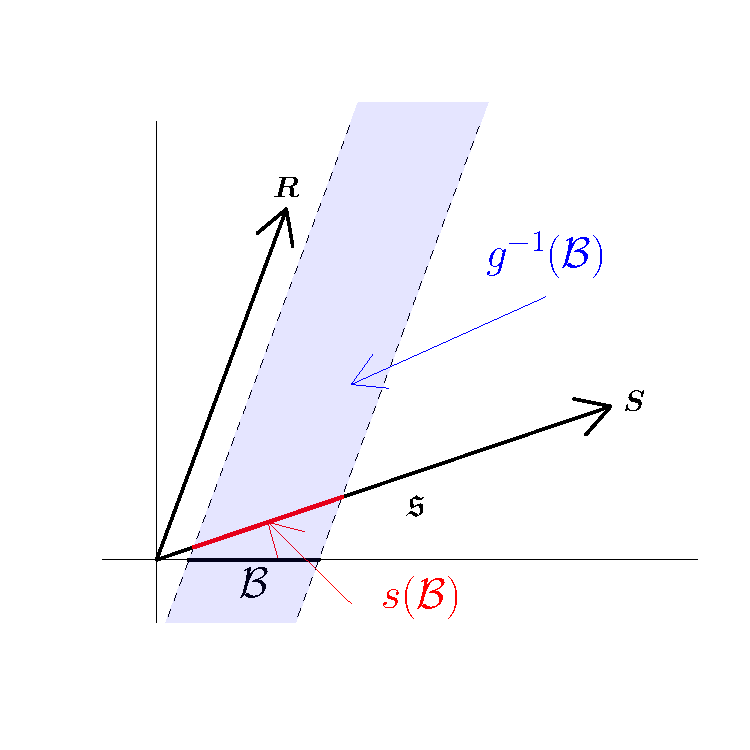
\includegraphics[width=0.6\textwidth]{Figs/probforerec_schematic.pdf}
	\caption{Summary of probabilistic forecast reconciliation. The probability that $\bm{y}_{t+h}$ lies in the red line segment under the reconciled probabilistic forecast is defined to be equal to the probability that $\bm{y}_{t+h}$ lies in the shaded blue area under the unreconciled probabilistic forecast. Note that since the smallest possible hierarchy involves three dimensions, this figure is only a schematic.}\label{fig:probfr_sch}
\end{figure}

\section{Construction of Reconciled Distribution} \label{sec:AnalyticalSolution}

In this section we derive theoretical results on how distributions on $\mathbb{R}^n$ can be reconciled to a distribution on $\mathfrak{s}$.  In section~\ref{sec:andens} we show how this can be achieved analytically by a change of coordinates and marginalisation when the density is available.  In section~\ref{sec:elliptical} we explore this result further in the specific case of elliptical distributions. In section~\ref{sec:SampleSolution} we consider reconciliation in the case where the density may be unavailable but it is possible to draw a sample from the base probabilistic forecast distribution.  Throughout we restrict our attention to linear reconciliation. 

\subsection{Analytical derivation of reconciled densities}\label{sec:andens}

The following theorem shows how a reconciled density can be derived from any base probabilistic forecast on $\mathbb{R}^n$.

\begin{theo}[Reconciled density of bottom-level]\label{theo:bottomdens}
	Consider the case where reconciliation is carried out using a composition of linear mappings $s\circ g$ where $g$ combines information from all levels of the base forecast into a new density for the bottom-level.  The density of the bottom-level series under the reconciled distribution is
	\[
	\tilde{f}_{\bm{b}}(\bm{b})=|\bm{G^*}|\int \hat{f}(\bm{G}^{-}{\bm b}+\bm{G}_\perp {\bm a})d\bm{a}\,,
	\]
	where $\hat{f}$ is the density of the incoherent base probabilistic forecast, $\bm{G^-}$ is an $n\times m$ generalised inverse of $\bm{G}$ such that $\bm{G}\bm{G}^-=\bm{I}$, $\bm{G_\perp}$ is an $n\times (n-m)$ orthogonal complement to $\bm{G}$ such that $\bm{G}\bm{G}_\perp=\bm{0}$, $\bm{G^*}=\left(\bm{G}^-\,\vdots\,\bm{G}_\perp\right)$, and $\bm{b}$ and $\bm{a}$ are obtained via the change of variables
	\[
	\bm{y}=\bm{G^*}\begin{pmatrix}\bm{b}\\\bm{a}\end{pmatrix}\,.
	\]
\end{theo}

\begin{proof}
	See Appendix \ref{app:Bottom&FullDens}.
\end{proof}

\begin{theo}[Reconciled density of full hierarchy]\label{theo:fulldens}
	Consider the case where a reconciled density for the bottom-level series has been obtained using Theorem~\ref{theo:bottomdens}.  The density of the full hierarchy under the reconciled distribution is
	\[
	\tilde{f}_{\bm{y}}(\bm{y})=|\bm{S^*}|\tilde{f}_{\bm b}({\bm{S^-}\bm{y}})\mathbb{1}\left\{\bm{y}\in\mathfrak{s}\right\}\,,
	\]
	where $\mathbb{1}\left\{.\right\}$ equals $1$ when the statement in braces is true and 0 otherwise and,
	\[\bm{S^*}=\begin{pmatrix}\bm{S}^-\\\bm{S}'_\perp\end{pmatrix}\,,\]
	and $\bm{S^-}$ is an $m\times n$ generalised inverse of $\bm{S}$ such that $\bm{S}^-\bm{S}=\bm{I}$, $\bm{S_\perp}$ is an $n\times (n-m)$ orthogonal complement to $\bm{S}$ such that $\bm{S}'_\perp\bm{S}=\bm{0}$.
\end{theo}

\begin{proof}
	See Appendix \ref{app:Bottom&FullDens}.
\end{proof}

\subsubsection*{Example: Gaussian Distribution}

Let the incoherent base forecasts be Gaussian with mean $\hat{\bm{\mu}}$, covariance matrix $\hat{\bm{\Sigma}}$ and density,
\begin{equation}
\hat{f}(\hat{y})=(2\pi)^{-n/2}|\hat{\bm{\Sigma}}|^{-1/2}\exp\left\{-\frac{1}{2}\left[({\bm{y}}-\hat{\bm{\mu}})'\hat{\bm{\Sigma}}^{-1}({\bm{y}}-\hat{\bm{\mu}})\right]\right\}\nonumber.
\end{equation}
Using Theorem~\ref{theo:bottomdens}, the reconciled density for the bottom-level series is given by,
\begin{equation}
\tilde{f}_{\bm{b}}(\bm{b})=\int(2\pi)^{-\frac{n}{2}}\Big|\hat{\bm{\Sigma}}\Big|^{-\frac{1}{2}}|\bm{G^*}|\exp\{-\frac{1}{2}q\}d{\bm a}\nonumber\,,
\end{equation}
where
\begin{align*}
	q& =
	\left(\bm{G}^*\bt-\hat{\bm{\mu}}\right)' \hat{\bm{\Sigma}}^{-1}\left(\bm{G}^*\bt-\hat{\bm{\mu}}\right)\\
	& =
	\left(\bt-\bm{G}^{*-1}\hat{\bm{\mu}}\right)' \Big[\bm{G}^{*-1}\hat{\bm{\Sigma}}\left(\bm{G}^{*-1}\right)'\Big]^{-1}
	\left(\bt-\bm{G}^{*-1}\hat{\bm{\mu}}\right)\,.
\end{align*}
Noting that
\[
\bm{G}^{*-1}=\begin{pmatrix}
\bm{G} \\\bm{G}_{\perp}^-
\end{pmatrix}\,,
\]
where $\bm{G}_{\perp}^-$ is an $(n-m)\times n$ matrix such that $\bm{G}_{\perp}^-\bm{G}_{\perp}=\bm{I}$, $q$ can be rearranged as
\[
 \left[\bt-\PQ\hat{\bm{\mu}}\right]' \left[\PQ\hat{\bm{\Sigma}}\PQ'\right]^{-1}\left[\bt-\PQ\hat{\bm{\mu}}\right]\,.
\]
After the change of variables, the density can be recognised as a multivariate Gaussian in $\bm{b}$ and $\bm{a}$.  The mean and covariance matrix for the margins of the first $m$ elements are $\bm{G}\hat{\bm{\mu}}$ and $\bm{G}\hat{\bm{\Sigma}}\bm{G}'$ respectively.  Marginalising out $\bm {a}$, the reconciled forecast for the bottom-level is $\tilde{\bm{b}} \sim \mathcal{N}(\bm{G}\hat{\bm{\mu}}, \bm{G}\hat{\bm{\Sigma}}\bm{G}')$.


\subsection{Elliptical distributions}\label{sec:elliptical}

More generally, consider linear reconciliation of the form $\psi(\hat{\bm{y}})=\bm{S}(\bm{d}+\bm{G}\hat{\bm{y}})$.  For an elliptical base probabilistic forecast, with location $\hat{\bm\mu}$ and scale $\hat{\bm\Sigma}$, the reconciled probabilistic forecast will also be elliptical with location $\tilde{\bm{\mu}}=\bm{S}(\bm{d}+\bm{G}\hat{\bm{\mu}})$ and scale   $\tilde{\bm{\Sigma}}=\bm{S}\bm{G}\hat{\bm{\Sigma}}\bm{G}'\bm{S}'$.  This is a consequence of the fact that elliptical distributions are closed under linear transformations and marginalisation. While the base and reconciled distribution may be of a different form they will both belong to the elliptical family.  This leads to the following result

\begin{theo}\label{theo:OptRec}
	Assume the true predictive distribution is elliptical with location ${\bm\mu}$ and scale ${\bm\Sigma}$.  Then for an elliptical base probabilistic forecast with arbitrary location $\hat{\bm\mu}$ and scale $\hat{\bm\Sigma}$, there exists $\bm{d}_{opt}$ and $\bm{G}_{opt}$ such that the true predictive distribution is recovered by reconciliation. 
\end{theo}
\begin{proof}
	First consider finding a $\bm{G}_{opt}$ for which the following holds, 
	\begin{equation*}
	\bm{\Sigma}=\bm{S}\bm{G}_{opt}\Sigma\bm{G}'_{opt}\bm{S}'\,.
	\end{equation*}
	This can be solved as $\bm{G}_{opt}={\bm{\Omega}}_0^{1/2}\hat{\bm \Sigma}^{-1/2}$, where $\hat{\bm \Sigma}^{1/2}$ is any matrix such that $\hat{\bm \Sigma}=\hat{\bm \Sigma}^{1/2}(\hat{\bm \Sigma}^{1/2})'$ (for example a Cholesky factor), ${\bm{\Omega}}_0^{1/2}({\bm{\Omega}}_0^{1/2})'={\bm\Omega}$ and ${\bm\Omega}$ is the true scale matrix for the bottom-level series. To ensure conformability of matrix multiplication, ${\bm{\Omega}}^{1/2}$ must be a $m\times n$ matrix so can be set to the Cholesky factor of ${\bm{\Omega}}$ augmented with an additional $n-m$ columns of zeros. To reconcile the location solve the following for $\bm{d}_{opt}$
	\begin{equation*}
	\bm{\mu}=\bm{S}(\bm{d}_{opt}+\bm{G}_{opt}\hat{\bm{\mu}})\,
	\end{equation*}
	which is given by $\bm{d}_{opt}=\bm{\beta}-\bm{G}_{opt}\hat{\bm\mu}$, where $\bm{\beta}$ is defined so that $\bm{\mu}=\bm{S}\bm{\beta}$. 
\end{proof}

While the above theorem is not feasible in practice (exploiting the result requires knowledge of $\bm{\mu}$ and $\bm{\Sigma}$), it does nonetheless have important consequences for the algorithm that we introduce in Section~\ref{sec:scoreoptSGD}. In particular, note that ${\bm S}{\bm G}_{opt}$ is not a projection matrix in general.  This implies that in the probabilistic forecasting setting, it is advised to include a translation $\bm{d}$ in the reconciliation procedure.  This holds even if the base forecasts are unbiased (i.e. $\hat{\bm{\mu}}=\bm{\mu}$) since in general ${\bm S}{\bm G}_{opt}\hat{\bm{\mu}}\neq\bm{\mu}$.  

Although ${\bm S}{\bm G}_0$ is not a projection matrix in general, there are some conditions under which it will be.  These are described by the following theorem.
\begin{theo}[Optimal Projection for Reconciliation]\label{theo:OptRecProj}
	Let $\hat{\bm{\Sigma}}$ be the scale matrix from an elliptical but incoherent base forecast and assume base forecasts are also unbiased.  When the true predictive is also elliptical, then this can be recovered via reconciliation using a projection if $\textrm{rank}(\hat{\bm{\Sigma}}-\bm{\Sigma})\leq n-m$.
\end{theo}
\begin{proof}
	See Appendix~\ref{app:OptRecProj}.
\end{proof}


\subsection{Simulation from a Reconciled Distribution}\label{sec:SampleSolution}

In practice it is often the case that samples are drawn from a probabilistic forecast since an analytical expression is either unavailable, or relies on unrealistic parametric assumptions.  A useful result is the following
\begin{theo}[Reconciled samples]
	Suppose that $\left(\hat{\bm y}^{[1]},\ldots,\hat{\bm y}^{[L]}\right)$ is a sample drawn from an incoherent probability measure $\hat{\nu}$.  Then $\left(\tilde{\bm y}^{[1]},\ldots,\tilde{\bm y}^{[L]}\right)$ where $\tilde{\bm y}^{[l]}:=\psi(\hat{\bm y}^{[l]})$ for all $l=1,\ldots,L$ is a sample drawn from the reconciled probability measure $\tilde{\nu}$ as defined in Definition~\ref{def:reconprob}
\end{theo}
\begin{proof}
	For any $\mathcal{A}\in\mathscr{F}_{\mathfrak{s}}$
\begin{align}
	\mbox{Pr}(\hat{{\bm y}}\in\psi^{-1}(\mathcal{A}))&=\underset{L\rightarrow\infty}{\lim}\sum\limits_{l=1}^L\mathbb{1}\left\{\hat{\bm y}^{[l]}\in\psi^{-1}(\mathcal{A})\right\}\nonumber\\
	&=\underset{L\rightarrow\infty}{\lim}\sum\limits_{l=1}^L\mathbb{1}\left\{\psi(\hat{\bm y}^{[l]})\in(\mathcal{A})\right\}\nonumber\\
	&=\mbox{Pr}(\tilde{{\bm y}}\in(\mathcal{A}))\nonumber
\end{align}
\end{proof}

This result implies that reconciling each member of a sample drawn from an incoherent distribution provides a sample from the reconciled distribution.  Such a strategy has already been used by \cite{JeoEtAl2019}, without formal justification.  This result allows coherent forecasts to be built in a general and modular fashion, the mechanism for simulating base forecasts is separated from the question of reconciliation.  This will become clear in the Simulation Study covered in Section~\ref{sec:simulations}.

%In the point forecasting setting it is common to generate forecasts from independent statistical models, allowing forecast reconciliation to be scaled up to large hierarchies.  Since a single point forecast is generated for each series there is no ambiguity as to how these should be stacked into a vector of base forecasts $\hat{\bm{y}}$.  This is no longer the case in the probabilistic setting where multiple draws are made for each series.  \cite{JeoEtAl2019} recommend some crude heuristics that can be used to form joint samples.  In Section~\ref{sec:drawbase} we provide an alternative based on resampling forecast errors. This provides a sample from a base probabilistic forecast. A sample from the reconciled distribution can be obtained by premultiplying these draws by $\bm{S}\bm{G}$. Strategies for choosing $\bm{G}$ are discussed in Section~\ref{sec:OptRec}.

%\subsection{Drawing base probabilistic forecasts}\label{sec:drawbase}
%
%The following method only requires that one-step ahead in-sample `forecasts' $\hat{y}_{i,t}$ can be computed for each series $i$.  These are not true forecasts since they are computed over the training data $t=1,\ldots,T$; for instance  $\hat{y}_{i,t}$ may be the fitted values of $E(y_{i,t}|y_{i,t-1})$ implied by some statistical model. Let the errors $e_{i,t} = y_{i,t} - \hat{y}_{i,t}$ be stacked in a $(n \times T)$ matrix $\bm{\mathcal{E}}:=\left\{e_{i,t}\right\}_{i=1,\dots,n,t=1,\dots,T}$.  When up to $H$ step ahead forecasts are required, we randomly select $H$ consecutive columns from $\bm{\mathcal{E}}$ to form $\bm{\mathcal{E}}^b$ and repeat for $b = 1,\dots,B$.  This preserves both serial correlation of errors as well as dependence across different series.
%
%The $\bm{\mathcal{E}}^b$ can then be used together with forecasts $\hat{\bm{y}}_{T+h}$ for $h=1,\ldots,H$ to recursively form $B$ sample paths of the full hierarchy.  As a simple example consider the case where each forecast comes from (the same) AR(1) model and $H=2$.  Then $\hat{{y}}^b_{i,T+1}=\phi{{y}}_{i,T}+e^b_{i,1}$ and $\hat{{y}}^b_{i,T+2}=\phi\hat{{y}}^b_{i,T+1}+e^b_{i,2}$ for each $i=1,\ldots,n$ and $b=1,\ldots,B$ and where $e^b_{i,h}$ is the element in row $i$ and column $h$ of $\bm{\mathcal{E}}^b$.  Each future path can be stacked into a vector $\hat{\bm{y}}^b_{T+h}:=(\hat{{y}}^b_{1,T+h},\ldots,\hat{{y}}^b_{n,T+h})'$ which in turn are stacked into a $n\times B$ matrix $\hat{\bm{\Upsilon}}_{T+h} = (\hat{\bm{y}}^1_{T+h},\dots,\hat{\bm{y}}^B_{T+h})$.
%
%As discussed previously, reconciling each draw from an incoherent distribution yields a sample from the reconciled distribution.  Therefore setting $\tilde{\bm{\Upsilon}}_{T+h} = \bm{SG}\hat{\bm{\Upsilon}}_{T+h}$ yields a matrix whose columns $\tilde{\bm{y}}^b_{T+h} := \bm{SG}\hat{\bm{y}}^b_{T+h}$ are a sample from the reconciled distribution.  In principle $\bm{G}$ matrices from popular point forecasting reconciliation methods can be used. In Section~\ref{sec:OptRec}, we propose a way to find an optimal $\bm{G}$ for reconciling future paths by minimising a proper multivariate scoring rule.

\section{Evaluation of Hierarchical Probabilistic Forecasts} \label{sec:evaluation}

An important issue in all forecasting problems is evaluating forecast accuracy. In the probabilistic setting, it is common to evaluate forecasts using proper scoring rules \citep[see][and references therein]{Gneiting2007,Gneiting2014}. Throughout, we follow the convention of negatively-oriented scoring rules such that smaller values of the score indicate more accurate forecasts.  In general, a scoring rule $K(.,.)$, is a function taking a probability measure as the first argument and a realisation as the second argument (although for ease of notation we will at times replace the probability measure with its associated density in the first argument). A scoring rule is {\em proper} if $\E_{Q}[K(Q,\bm{\omega})] \le \E_{Q}[K(P,{\bm\omega})]$ for all $P$, where $P$ is any member of some class of probability measures (densities), $Q$ is the true predictive and $\omega$ is a realisation. When this inequality is strict for all $P\neq Q$, the scoring rule is said to be {\em strictly proper}.

Since hierarchical forecasting is by its very nature a multivariate problem (the linear constraints affect all variables), our focus is on multivariate scoring rules.  Arguably the simplest and most common multivariate scoring rule is the log score. The log score simply involves evaluating the negative log density at the value of the realisation, $\text{LS}(P,\bm\omega)=-\log f(\bm\omega)$, where $f$ is the density associated with a distribution $P$.  The log score is more commonly used when a parametric form for the density is available, however  this density can also be approximated from a sample of values drawn from the probabilistic forecast \citep[see][]{Jordan2017}.

Alternatively there are a number of other multivariate scoring rules that are difficult to compute using the probabilistic forecast density alone, but can be approximated using a sample drawn from that density.  An example is the energy score (ES) \citep[see][for details]{szekely2003,Gneiting2007} which is multivariate generalisation of the popular Cumulative Rank Probability Score (CRPS).  The energy score is given by
\begin{equation}\label{eq:Energy_score}
\text{ES}(P,\bm{\omega}) =
\E_{P}
||{\bm{y}}-\bm{\omega}||^\alpha -\frac{1}{2}\E_{P}||\bm{y}-\bm{y}^*||^\alpha, \,\, \alpha \in (0,2]\,,
\end{equation}
where $\bm {y}$ and $\bm{y^*}$ are independent copies drawn from the distribution $P$, and we follow common convention by setting $\alpha=0.5$.  While the expectations in Equation~\ref{eq:Energy_score} may have no closed form, they can be easily approximated via Monte Carlo using a sample drawn from the probabilistic forecast.  Other scores with similar behaviour are kernel-based scores \citep{dawid2007,Gneiting2007} and the variogram score \citep{SCHEUERER2015}.

%The energy score has been criticised by \citet{Pinson2013a} for its low discriminative ability for incorrectly specified covariances.  The variogram score  \citep{SCHEUERER2015}, overcomes this issue and is defined as
%\begin{equation*}
%\text{VS}({P}, \bm{\omega}) = \displaystyle\sum_{i=1}^{n}\displaystyle\sum_{j=1}^{n}w_{ij}\left(|\omega_{i} - \omega_{j}|^p - E_{P} |{y}_{i}-{y}_{j}|^p\right)^2\,,
%\end{equation*}
%where $y_i$ and $y_j$ are the $i^{th}$ and $j^{th}$ elements of $\bm{y}\sim P$ and we follow common convention by setting $p=0.5$.

%In the context of probabilistic forecast reconciliation there could be two motivations for using scoring rules. The first is to compare incoherent base probabilistic forecasts to their reconciled counterparts, to see whether reconciliation improves forecast accuracy. The second is to compare two reconciled probabilistic forecasts to one another, to evaluate which choice of $\bm{G}$ performs best in practice.

\subsection{The Log Score for Hierarchical Time Series}

When a expression for the density of an incoherent base forecast is available, Section~\ref{sec:AnalyticalSolution} describes how the density of a reconciled forecast can be recovered.  With both densities available, the log score is natural and straightforward scoring rule to use.  However, the following theorem shows that the log score is improper in the setting of comparing incoherent to coherent forecasts.

\begin{theo}[Impropriety of log score]\label{theo:logS_improp}
	When the true data generating process is coherent, then the log score is improper with respect to the class of incoherent measures.
\end{theo}

\begin{proof}
	See Appendix \ref{app:logS_improp}.
\end{proof}

As a result of Theorem~\ref{theo:logS_improp} we recommend avoiding the log score when comparing reconciled and unreconciled probabilistic forecasts.

If a probabilistic forecast is available for any $m$ series, then a probabilistic forecast for the full hierarchy can be derived.  Definition~\ref{def:cohprob} provides an example using the bottom-level series. This suggests that it may be adequate to merely compare two coherent forecasts to one another using the bottom-level series only. This is true for the log score.

Consider a coherent probabilistic forecast with density $\tilde{f}_{\bm{y}}$ for the full hierarchy and $\tilde{f}_{\bm{b}}$ for the bottom-level series. By Theorem~\ref{theo:fulldens}, $\tilde{f}_{\bm{y}}(\bm{y})=|\bm{S}^*|\tilde{f}_{\bm{b}}(\bm{S}^-\bm{y})\mathbb{1}{\bm{y}\in\mathfrak{s}}$.  Any realisation $\bm{y}^*$ will lie on the coherent subspace and can be written as $\bm{S}\bm{b}^*$.  The expression for the log score is therefore
\begin{align}
\text{LS}(\tilde{f}_{\bm y},\bm{y}^*)&=-\log\left(|\bm{S}^*|\tilde{f}_{\bm{b}}(\bm{S}^-\bm{S}\bm{b}^*)\right)\nonumber\\
&=-\log|\bm{S}^*|-\log \tilde{f}_{\bm{b}}(\bm{b}^*).\nonumber
\end{align}
For coherent densities, the log score for the full hierarchy differs from the log score for the bottom-level series only by $-\log|\bm{S}^*|$. This term is independent from the choice of ${\bm G}$. As such, rankings of different reconciliation methods using the log score for the full hierarchy will not change if only the bottom-level series is used.

The same property does not hold for all scores. For example, the energy score is invariant under orthogonal transformations \citep{Szekely2013} but not under linear transformations in general. Therefore it is possible for one method to outperform another when energy score is calculated using the full hierarchy, but for these ranking to reverse if only bottom-level series are considered.  We therefore recommend computing the energy score using the full hierarchy.  The properties of multivariate scoring rules in the context of evaluating reconciled probabilistic forecasts are summarised in Table~\ref{tab:prop}.

\begin{table}
	\caption{Properties of scoring rules for reconciled probabilistic forecasts.}\label{tab:ScoringRulesProperties}
	\centering
	\begin{tabular}{lll}\hline
		Scoring Rule& Coherent v Incoherent &Coherent v Coherent\\
		\hline
		Log Score & Not proper & Ordering preserved if compared \\ && using bottom-level only\\
		Energy Score & Proper & Full hierarchy should be used\\
		\hline
	\end{tabular}
	
	\label{tab:prop}
\end{table}

\section{Score Optimal Reconciliation}\label{sec:scoreoptSGD}

We now propose an algorithm for finding reconciliation weights by optimising the total score.  We will consider the special case of the energy score, however the algorithm can be generalised to any score that is computed by sample from the probabilistic forecast, including the variogram and kernel score.  We consider linear reconciliation of the form $\tilde{\bm{y}}=\psi_{\bm{\gamma}}({\bm{\hat{y}}})={\bm{S}}\left(\bm{d}+\bm{G}{\bm{\hat{y}}}\right)$, where ${\bm\gamma}:=\left(\bm{d},vec(\bm{G})\right)$. This allows for more flexibility than a projection, which implies the constraints $\bm{d}=\bm{0}$ and $\bm{G}\bm{S}=\bm{I}$.  This added flexibility is motivated by Theorem~\ref{theo:OptRec} which shows that projections in general are not guaranteed to recover the true predictive distribution even in the elliptical case. When making a $h$-step ahead forecast at time $T$ the objective used to determine an optimal value of $\bm{\gamma}$ is the total energy score based on in-sample information given by:
\begin{equation}
\mathcal{E}\left(\bm{\gamma}\right)=\sum\limits_{t=1}^{T-h} \textit{ES}(\tilde{f}^{\bm{\gamma}}_{t+h|t},\bm{y}_{t+1})\,,
\label{eq:tes}
\end{equation} 
where $\tilde{f}^{\bm{\bm{\gamma}}}_{t+h|t}$ is probabilistic forecast for $\bm{y}_{t+h}$ made at time $t$ and reconciled with respect to $\psi_{\bm{\gamma}}(.)$.  

One of the challenges to optimising this objective function is that there is, in general, no closed form expression for the energy score.  However, it can be easily approximated by Monte Carlo as
\begin{equation*}
\hat{\mathcal{E}}\left(\bm{\gamma}\right)=\sum\limits_{t=1}^{T-h}\left[\frac{1}{Q}\left(\sum\limits_{q=1}^{Q}||\tilde{\bm{y}}^{[q]}_{t+h|t}-\bm{y}_{t+h}||-\frac{1}{2}||\tilde{\bm{y}}_{t+h|t}^{[q]}-\tilde{\bm{y}}^{*[q]}_{t+h|t}||\right)\right]\,,
\label{eq:obj_mc}
\end{equation*} 
where $\tilde{\bm{y}}^{[q]}_{t+h|t}=\bm{S}\left(\bm{d}+\bm{G}{\hat{\bm{y}}}^{[q]}_{t+h|t}\right)$, $\tilde{\bm{y}}^{*[q]}_{t+h|t}=\bm{S}\left(\bm{d}+\bm{G}{\hat{\bm{y}}}^{*[q]}_{t+h|t}\right)$ and ${\hat{\bm{y}}}^{[q]}_{t+h|t},{\hat{\bm{y}}}^{*[q]}_{t+h|t}\overset{iid}{\sim} \hat{f}_{t+h|t}$ for $q=1,\ldots,Q$, and $t=1,\ldots,T-h$.  Therefore the objective function can be optimised by Stochastic Gradient Descent (SGD). The SGD technique has become increasingly popular in machine learning and statistics over the past decade having been applied to training neural networks \citep{bottou2010} and Variational Bayes \citep{kingma2013}.  The method requires an estimate of the gradient $\partial\hat{\mathcal{E}}/\partial{\gamma}$ which is computed by automatically differentiating Equation~\ref{eq:obj_mc} using the header only C++ library of the Stan project~\citep{carpenter2015}.  The learning rates used for SGD are those of the Adam method \citep[see][for details]{kingma2014}.  The tuning parameters are set as $\eta=0.001$, $\beta_1=0.9$, $\beta_2=0.999$ and $\epsilon=1\times 10^{-8}$, which are the values recommended by \cite{kingma2014} and used in popular software packages such as TensorFlow, Keras and Torch amongst others.  Convergence is achieved when the change in all gradients is less than 10\% of the step size $\eta$.  The full procedure is described in Algorithm~\ref{alg:scoreopt} for one step ahead forecasts and is implemented in the R package \texttt{ProbReco} publicly available at the GitHub repository \texttt{anastasiospanagiotelis/ProbReco}.

\begin{algorithm}
	\caption{SGD with Adam for score optimal reconciliation (one-step ahead forecasts).  The initial value of $\bm{\gamma}$ is given by OLS reconciliation.  Steps 9-14 are the standard steps for SGD with Adam.  Squaring $\bm{g}_j$ in step 11 and division in step 14 are element-wise operations.}\label{alg:scoreopt}.
	\begin{algorithmic}[1]
		\Procedure{ScoreOpt}{$\hat{f}_{2|1},\ldots,\hat{f}_{T|T-1|1}$, $\bm{y}_1,\ldots,\bm{y}_T$, $\beta_1$,$\beta_2$,$\epsilon$,$\eta$}.
		\For{t=1:T-1}
		  \State Find base forecasts $\hat{f}_{t+1|t}$ using $t-S,t-S+1,\ldots t$ as training data.		
		\EndFor
		\State Initialise $\bm{m}_0=\bm{0}, \bm{v}_0=\bm{0}$ and $\bm{\gamma}_0=\left(\bm{0},vec\left((\bm{S}'\bm{S})^{-1}\bm{S}'\right)\right)$ 
		\For{j = 1,2,3,\ldots up to convergence}
		\State Draw ${\hat{\bm{y}}}^{[q]}_{t+1|t},{\hat{\bm{y}}}^{*[q]}_{t+1|t}\sim \hat{f}_{t+1|t}$ for $q=1,\ldots,Q$, $t=1,\ldots T-1$.
		\State Compute $\tilde{\bm{y}}^{[q]}_{t+1|t}$ and $\tilde{\bm{y}}^{*[q]}_{t+1|t}$ for $q=1,\ldots,Q$, $t=1,\ldots T-1$ using $\bm{\gamma}_{j-1}$.
		\State $\bm{g}_j \gets \left.\partial\hat{\mathcal{E}}/\partial{\bm{\gamma}}\right|_{\bm{\gamma}=\bm{\gamma}_{j-1}}$ \Comment{Compute gradient}
		\State $\bm{m}_j\gets\beta_1\bm{m}_{j-1}+(1-\beta_1)\bm{g}_j$ \Comment{Moving average of gradient}
		\State $\bm{v}_j\gets\beta_2\bm{v}_{j-1}+(1-\beta_2)\bm{g}^2_j$ \Comment{Moving average of squared gradient}
		\State $\hat{\bm{m}}_j\gets \bm{m}_j/(1-\beta_1^j)$ \Comment{Bias correct}
		\State $\hat{\bm{v}}_j\gets \bm{v}_j/(1-\beta_2^j)$ \Comment{Bias correct}
		\State $\bm{\gamma}_j\gets\bm{\gamma}_{j-1}+\eta\frac{\hat{\bm{m}}_j}{(\hat{\bm{v}}_j+\epsilon)}$ \Comment{Update weights}
		\EndFor
		\State Set the reconciled forecast as $\tilde{f}^{\bm{\gamma}_{opt}}_{T+1|T}$ where $\bm{\gamma}_{opt}$ is the converged value of $\bm{\gamma}$.
		\EndProcedure
	\end{algorithmic}
\end{algorithm}

While Algorithm~\ref{alg:scoreopt} is not the first instance of calibrating parameters by optimising scoring rules \citep[see][for an example]{gneiting2005}, to the best of our knowledge it is the first instance of doing so using SGD and the first application to forecast reconciliation.  It is amenable to parallel computing architectures, the loop beginning at line 2 of the pseudocode of Algorithm~\ref{alg:scoreopt} can be done in parallel as can the computation of the gradient.  Finally, the total score in Equation~\ref{eq:tes} can be replaced with a weighted sum where appropriate, for instance weights that decay for scores computed further in the past will favour choices of $\bm{\gamma}$ that produced better forecasting performance for more recent forecast windows.

\section{Simulations}\label{sec:simulations}

The aim of the simulations that follow is to demonstrate probabilistic forecast reconciliation including the algorithm discussed in Section~\ref{sec:scoreoptSGD}.  A number of different data generating processes, models and approaches to obtain base forecasts are considered. 

\begin{itemize}
	\item describe all DGPS stationary/non-stationary gaussian/nongaussian and models ARIMA/ETS
	
	\item Explain all 4 ways of doing base forecasts independent/joint gaussian/non-gaussian
	
	\item Reconiciliation Methods: Base, Ben Taieb et al (?), Jeon et all. Projections (BU, OLS, WLS, MinT) Score Optimal.
	
	\item Completely rewrite results
\end{itemize}

\subsection{Data Generating Processes}\label{sec:dgp}

The data generating process we consider corresponds to the 3-level hierarchical structure presented in Figure \ref{fig:twoL-hier}. Bottom-level series are first generated from ARIMA$(p,d,q)$ processes, which are in-turn aggregated to form the middle and top-level series. The orders $p$, and $d$ are randomly selected from $\{1,2\}$ for each bottom level series. Both a non-stationary case where $d$ is randomly chosen for each bottom level $\{0,1\}$ and a stationary case where $d$ is set to zero for all bottom level series.  The parameters for the AR and MA components are randomly and uniformly generated from $[0.3,0.5]$ and $[0.3,0.7]$ respectively where in the case of the stationary series these are only accepted if they belong to the stationary and invertible region.

We consider a multivariate Gaussian and a non-Gaussian setting for the errors driving the ARIMA processes. More specifically the non-Gaussian errors are drawn from a meta-distribution of a Gumbel copula with $\textrm{Beta}(1,3)$ margins. After simulating from the ARIMA models, additional noise is added to ensure bottom level series have a lower signal-to-noise ratio that top level series with specific details provided in Appendix \ref{app:DGP}.  This yields a total of four data generating processes (DGPs) for each combination of stationary/non-stationary and Gaussian/non-Gaussian.  For each series we generate 2000 observations from which the first 500 are ignored to avoid the impact of initial values. 

%All forecasts are evaluated using a rolling window with a training sample of 500. This yields 1,000 probabilistic forecasts for evaluation. The predictive accuracy of the alternative methods is evaluated using the scoring rules presented in Section~\ref{sec:evaluation}. Results are reported in terms of skill scores, i.e., the percentage improvement of a probabilistic forecast over a reference method. A positive (negative) value indicates a percentage gain (loss) in forecast accuracy over the reference method.

\subsection{Modelling and Base Forecasts}

We fit univariate ARIMA and exponential smoothing (ETS) models to each series using the \verb|auto.arima()| and \verb|ets()| functions in the \verb|fable| package \citep{Rfable} in R \citep{Rcore}.  Note that the order of the ARIMA models is not set to the true order but is chosen using the algorithm of \cite{hynkan2007}, allowing for the possibility of misspecification.  Indeed, an advantage of forecast reconciliation is the ability to down-weight the forecasts of series within the hierarchy that come from misspecified models.  For each series and model, base probabilistic forecasts are constructed in four different ways.  Letting $\hat{\bm y}_{t+h|h}L=\hat{y}_{1,t+h|h},\ldots,\hat{y}_{n,t+h|h}$ where $\hat{y}_{i,t+h|h}$ is the point forecast for series $i$ and $e_{i,t}$ be residuals stacked in a $(n \times T)$ matrix $\bm{E}:=\left\{e_{i,t}\right\}_{i=1,\dots,n,t=1,\dots,T}$, these are:

\begin{enumerate}[label=(\alph*)]
	\item The base probabilistic forecast is made up of independent Gaussian distributions with the forecast mean and variance of variable $i$ given by $\hat{y}_{i,t+h|h}$ and $\hat{\sigma}^2_{i,t+h|h}$,
	\item The base probabilistic forecast is multivariate Gaussian distributions with the forecast mean $\hat{\bm{y}}_{t+h|h}$ and variance covariance matrix $\hat{\bm\Sigma}$, where $\hat{\bm\Sigma}$ is the variance covariance matrix of residuals,
	\item A draw from the base probabilistic forecast is made independently for each variable as $\hat{y}_{i,t+h|h}+e_{i,s}$ where $s$ is drawn randomly (with replacement) from $1,2,\ldots, T$, and
	\item A draw from the joint probabilistic is made as $\hat{\bm y}_{t+h|h}+\bm{e}_{s}$ where $\bm{e}_{s}$ is the $s^{th}$ column of $\bm{E}$, where $s$ is drawn randomly (with replacement) from $1,2,\ldots, T$.
\end{enumerate}

We restrict our attention to the case of $h=1$ although these methods can be generalised to larger $h$ using the recursive method \citep{FPP2018}.  For multi-step ahead forecasts, methods (c) and (d) should sample in blocks to preserve serial dependence in the residuals.

\subsection{Reconciliation}

For each DGP, model and method for obtaining base forecasts, reconciled probabilistic forecasts are obtained using each of the following techniques.

\begin{itemize}
	\item \textbf{Base:} The base forecasts with no reconciliation.
	\item \textbf{JPP:} The best method of \cite{JeoEtAl2019}.  This is equivalent to reconcile quantiles.  A sample is drawn from the base forecast, these are ranked, one variable at a time (so that the smallest value drawn from each variable are put together, etc.).  These are then pre-multipled by $\bm{S}\left(\bm{S}'\bm{W}\bm{S}\right)^{-1}\bm{S}'\bm{W}$ where $\bm{W}$ is a diagonal matrix with elements ($1/4^2$,$1/2^2$,$1/2^2$,$1$,$1$,$1$,$1$).  These are the squared reciprocals of the number of bottom level series used to form an aggregate.
	\item \textbf{BTTH} The method of \cite{Taieb2017}.  This is a method whereby draws from the probabilistic forecasts of the bottom level series are permuted so that they have the same empirical copula as the residuals.  These are then aggregated to form a sample from the distribution of all series.  The mean is adjusted to be equivalent to the mean that would be obtained using the MinT shrink method \cite{WicEtAl2019} described in Table~\ref{tab:recomethods}. 
	\item \textbf{BottomUp:} Reconciliation via premultiplication by $\bm{S}\bm{G}$ where $\bm{G}=\left(\bm{0}_{m\times(n-m)},\bm{I}_{m\times m}\right)$ 
	\item \textbf{OLS:} Reconciliation via premultiplication by $\bm{S}\left(\bm{S}'\bm{S}\right)^{-1}\bm{S}'$,
	\item \textbf{WLS:} Reconciliation via premultiplication by the same matrix used in \cite{JeoEtAl2019} but without any reordering of the draws,
	\item \textbf{MinT:} Reconciliation via premultiplication by the same matrix used in \cite{WicEtAl2019} but applied to probabilistic rather than point forecasting,
	\item \textbf{ScoreOpt:} The algorithm described in Section~\ref{sec:scoreoptSGD}.
\end{itemize}

Note JPP and BTTH are two methods previously existing in the literature. The methods BottomUp, OLS, WLS and MinT have been used extensively in the point forecasting literature but their application to probabilistic forecasting for general base forecasts is novel.

\subsection{Results for Gaussian probabilistic forecasts}\label{sec:SimAnalysticalResults}

%We assume a Gaussian predictive density for the simulated hierarchical time series, i.e., $\hat{\bm{y}}\sim N(\hat{\bm{\mu}},\hat{\bm{\Sigma}})$. The analytical tractability of the normal distribution allows for evaluation using all scoring rules (including the log-score). $\hat{\bm{\mu}}$ is given by the mean of the incoherent base probabilistic forecasts. We estimate $\hat{\bm{\Sigma}}$ from the in-sample one-step ahead forecast errors using the shrinkage estimator of \citet{Schafer2005} (as the one presented in Table \ref{tab:ReconMethods}). Coherent probabilistic forecasts are then generated as $\tilde{\bm{y}}\sim N(\bm{S}\bm{G}\hat{\bm{\mu}},\bm{S}\bm{G}\hat{\bm{\Sigma}}\bm{G}'\bm{S}')$ where ${\bm G}=(\bm{R}_{\perp}'\bm{S})^{-1}\bm{R}_{\perp}'$ and $\bm{R}'_\bot=\bm{S}'\bm{W}^{-1}$ for the different choices of $\bm{W}$ as presented in Table \ref{tab:ReconMethods}.

Table~\ref{tab:SimAnalyticalMulti} summarises the forecasting performance of incoherent, bottom-up, OLS, WLS and two MinT reconciliation methods using log score, energy score and variogram score. The top panel refers to the Gaussian DGP whereas the bottom panel refers to the non-Gaussian DGP. Recall that the log score is improper with respect to incoherent forecasts. Hence, we calculate the skill scores with reference to the bottom-up forecasts in all cases leaving blank the cells for log score of the incoherent forecasts. Further, all log scores are evaluated on the basis of bottom-level series only, as these differ from the log scores for the full hierarchy by a fixed constant. Please refer to Table \ref{tab:ScoringRulesProperties} for further explanations.

All reconciliation approaches that use information from all levels of the hierarchy improve on the incoherent base forecasts. The bottom-up that uses information only from the bottom-level does not improve on the base incoherent forecasts when considering the Energy Score. Overall, the MinT methods provide the most improvement over the incoherent base forecasts irrespective of the scoring rule or the nature of the DGP.

Tables~\ref{tab:SimAnalyticalUni} (and \ref{tab:SimAnalyticalUni_h2} and \ref{tab:SimAnalyticalUni_h3} in Appendix \ref{app:AnalysticalSolMargins} break down the forecasting performance of the different methods by considering univariate scores on each individual margin. Univariate log score and CRPS are considered, while skill scores are computed with the incoherent forecasts as a reference. When broken down in this fashion, irrespective of DGP, the methods based on MinT perform best for most series and outperform bottom-up forecasts in almost all cases.

\begin{table}[H]
	\caption{Forecast evaluation of hierarchical probabilistic forecasts for $h=1, 2$ and $3$ steps ahead. Entries show the percentage (\%) skill score with reference to the bottom-up method. A positive (negative) entry shows a gain (loss) in forecast accuracy over the reference method. The top panel shows the results from the Gaussian DGP while the bottom panel shows the results from the non-Gaussian DGP. The Log Score entries are based on the joint forecast distribution for the bottom-level (see Table \ref{tab:ScoringRulesProperties} for a further explanation), while the Energy and Variogram skill scores are based on the joint forecast distribution across the entire hierarchy.}
\label{tab:SimAnalyticalMulti}
	\centering
	\resizebox{\linewidth}{!}{
		\begin{tabular}{lccccccccc}
			\toprule
			\multicolumn{1}{c}{} & \multicolumn{3}{c}{Log Score (\%)} & \multicolumn{3}{c}{Energy Score (\%)} & \multicolumn{3}{c}{Variogram Score (\%)} \\
			\cmidrule(lr){2-4} \cmidrule(lr){5-7} \cmidrule(lr){8-10}
			$h$ & 1 & 2 & 3 & 1 & 2 & 3 & 1 & 2 & 3\\
			\toprule
			\multicolumn{10}{c}{Gaussian DGP}\\
			\toprule
			Incoherent base & & & & 12.46 & 9.58 & 7.19 & 4.91 & 5.89 & 6.02\\
			Bottom-up & 0.00 & 0.00 & 0.00 & 0.00 & 0.00 & 0.00 & 0.00 & 0.00 & 0.00\\
			OLS & 5.56 & -1.55 & -10.74 & 16.83 & 13.43 & 10.44 & 9.17 & 9.63 & 9.02\\
			WLS & 6.66 & -2.79 & -15.79 & 19.06 & 15.34 & 11.88 & 11.52 & 12.24 & 11.62\\
			MinT(Sample) & \textbf{7.73} & -2.59 & -17.07 & \textbf{21.55} & \textbf{17.36} & 13.60 & \textbf{15.74} & 15.75 & 15.51\\
			MinT(Shrink) & 7.70 & -2.63 & -17.12 & 21.44 & 17.33 & 13.60 & 15.65 & \textbf{15.98} & \textbf{15.58}\\
			Optimal & 5.31 & \textbf{2.86} &\textbf{ 4.28} & 8.08 & 13.75 & \textbf{15.10} & -14.12 & 3.60 & 6.57\\
			%		\midrule
			%		\textit{Bottom up} & $\mathbi{11.9}$ & $\mathbi{5.49}$ & $\mathbi{2.25}$ & $\mathbi{14.3}$ & $\mathbi{6.37}$ & $\mathbi{2.40}$ & $\mathbi{17.00}$ & $\mathbi{7.35}$ & $\mathbi{2.56}$\\
			\toprule
			\multicolumn{10}{c}{Non-Gaussian DGP}\\
			\toprule
			Incoherent base & & & & 7.18 & 7.37 & 7.13 & -0.44 & -0.35 & -0.22\\
			Bottom-up & 0.00 & 0.00 & 0.00 & 0.00 & 0.00 & 0.00 & 0.00 & 0.00 & 0.00\\
			OLS & 12.11 & 7.48 & -1.61 & 9.73 & 10.28 & 10.18 & 0.50 & 0.52 & 0.87\\
			WLS & 19.80 & 1.56 & -39.14 & 11.20 & 12.00 & 11.52 & 0.49 & 0.46 & 0.62\\
			MinT(Sample) & \textbf{22.89} & 4.69 & -36.42 & \textbf{12.94} & 14.07 & \textbf{13.44} & \textbf{1.78} & 2.16 & 2.07\\
			MinT(Shrink) & 22.67 & 4.43 & -36.76 & 12.92 & \textbf{14.13} & 13.39 & 1.63 & \textbf{2.18} & \textbf{2.20}\\
			Optimal & 19.15 & \textbf{9.26} & -4.11 & -3.31 & 3.48 & 2.41 & -27.79 & -19.37 & -22.70\\
			\bottomrule
		\end{tabular}
	}
\end{table}


\begin{table}[H]
	\caption{Forecast evaluation of univariate hierarchical probabilistic forecasts for $h=1$-step ahead. Entries show the percentage (\%) skill score base on the Log Score and CRPS with reference to the incoherent base forecasts. A positive (negative) entry shows a gain (loss) in forecast accuracy over the incoherent base forecasts. The left panel shows the results from the Gaussian DGP while the right panel shows the results from the non-Gaussian DGP.}
\label{tab:SimAnalyticalUni}
	\centering
	\resizebox{\linewidth}{!}{
		\begin{tabular}{lcccccccccccccc}
			\toprule
			\multicolumn{1}{c}{ } & \multicolumn{7}{c}{Gaussian} & \multicolumn{7}{c}{Non-Gaussian}\\
			\cmidrule(lr){2-8} \cmidrule(lr){9-15}
						
			Series & Tot & A & B & AA & AB & BA & BB & Tot & A & B & AA & AB & BA & BB \\
			\toprule
			\multicolumn{15}{c}{Log Score (\%)}\\
			\toprule
			Incoherent Base & 0.00 & 0.00 & 0.00 & 0.00 & 0.00 & 0.00 & 0.00 & 0.00 & 0.00 & 0.00 & 0.00 & 0.00 & 0.00 & 0.00\\
			Bottom up & -29.59 & -2.99 & -4.24 & 0.00 & 0.00 & -5.94 & 8.11 & -263.36 & -0.72 & -3.54 & 0.00 & 0.00 & -0.81 & -12.22\\
			OLS & 12.26 & 2.51 & 0.43 & 1.80 & 1.06 & -3.41 & 7.59 & 49.53 & 0.38 & 2.58 & -1.40 & 3.51 & 0.55 & -11.33\\
			WLS & \textbf{16.10} & -3.73 & -14.04 & 2.34 & 1.27 & -3.08 & 0.45 & 75.34 & 4.86 & -269.27 & -1.38 & 3.36 & 0.91 & -5.38\\
			MinT(Sample) & -0.07 & \textbf{4.80} & \textbf{0.54} & \textbf{3.86} & \textbf{2.55} & -2.34 & \textbf{8.20} & 0.24 & 0.44 & \textbf{5.18} & \textbf{0.61} & 3.73 & \textbf{2.46} & -10.21\\
			MinT(Shrink) & -0.05 & \textbf{4.80} & \textbf{0.54} & 3.65 & 2.48 & -2.36 & \textbf{8.20} & 0.27 & \textbf{0.45} & \textbf{5.18} & -1.42 & \textbf{3.75} & 2.30 & -10.32\\
			Optimal & 13.86 & 1.37 & -18.41 & -0.28 & -1.75 & -6.75 & 4.13 & \textbf{70.23} & -5.37 & -287.34 & -6.99 & -2.02 & -4.07 & -17.38\\
			\hline
			
			\toprule
			\multicolumn{15}{c}{CRPS (\%)}\\
			\toprule
			
			Incoherent Base & 0.00 & 0.00 & 0.00 & 0.00 & 0.00 & 0.00 & 0.00 & 0.00 & 0.00 & 0.00 & 0.00 & 0.00 & 0.00 & 0.00\\
			Bottom up & -134.06 & -10.99 & -15.42 & -0.05 & -0.14 & -21.39 & 25.07 & -485.01 & -1.41 & -9.35 & -0.01 & 0.08 & -1.85 & -36.37\\
			OLS & 35.17 & 8.45 & 1.17 & 6.49 & 3.07 & -11.45 & 23.77 & 74.22 & 1.30 & 6.77 & -3.85 & 9.21 & 1.82 & -33.37\\
			WLS & \textbf{43.24} & -13.62 & -50.06 & 8.16 & 3.82 & -10.32 & 1.12 & 87.17 & \textbf{12.20} & -503.54 & -3.90 & 8.85 & 2.85 & -16.01\\
			MinT(Sample) & -0.20 & \textbf{15.84} & \textbf{1.75} & \textbf{12.48} & \textbf{7.98} & -7.53 & \textbf{25.38} & 0.24 & 1.34 & 12.79 & \textbf{1.39} & 9.67 & \textbf{6.70} & -29.83\\
			MinT(Shrink) & -0.19 & 15.69 & 1.59 & 12.06 & 7.76 & -7.61 & 25.35 & 0.26 & 1.52 & \textbf{12.88} & -3.82 & \textbf{9.84}& 6.38 & -30.00\\
			Optimal & 37.22 & 3.37 & -74.40 & -2.85 & -8.50 & -27.27 & 11.28 & \textbf{85.14} & -16.83 & -599.74 & -21.16 & -7.42 & -13.08 & -55.62\\
			\bottomrule
		\end{tabular}
	}
\end{table}

\subsection{Results for non-Gaussian probabilistic forecast} \label{sec:SimSamplingResults}


%Bootstrap approach: Generate 2102 data points for each series. Ignoring first 500 observations to avoid the impact of initial values. Choose 600 observations for outer rolling window and follow the steps in the algorithm to generate reconciled probabilistic forecasts for  h = 1, 2 and 3 steps ahead forecast horizons.  Replicate the process for 1000 times by rolling the window one step at a time. This yields 1000 forecast distributions for evaluation for all forecast horizons.

%\subsection{Simulation setup for non-parametric solution}

%We now implement the non-parametric approach introduced in Section \ref{sec:SampleSolution}. Our main focus in this study is to compare different reconciliation methods to optimal reconciliation. We narrow down the study to find optimality with respect to energy score. Following equation (\ref{eq:Energy_score}) for samples from the probability distribution and for $\alpha = 1$, we can rewrite the objective function in (\ref{eq:Obj_func_apprx}) as,

%\begin{equation}\label{eq:Obj_func_apprx_ES}
%\operatornamewithlimits{argmin}_{\bm{G}} \frac{1}{N}\sum_{j=1}^{N}\left\{\frac{1}{B}\sum_{b=1}^{B}||\bm{SG}_h\bm{y}_{T+h,j}^b -\bm{y}_{T+h,j}||-\frac{1}{2(B-1)}\sum_{b=1}^{B-1}||\bm{SG}_h(\bm{y}_{T+h,j}^b -\bm{y}_{T+h,j}^{b+1})||\right\}
%\end{equation}

%First we generate $2500$ data points for each series in the hierarchy using the same DGP discussed in Section \ref{sec:simulations}. Following the algorithm explained in Section \ref{sec:OptRec}, we choose $L=600$ observations for outer rolling window and $T=500$ observations for inner rolling window. We fit univariate ARIMA models using \verb|auto.arima()| function and generate $B=1000$ of $h=1$ to $3$ steps-ahead incoherent bootstrapped future paths following steps 2 and 3. We repeat these steps for $N=100$ times by moving the inner window one step at a time. Following step 6, we then estimate $\bm{G}_h^{Opt}$. We use numerical optimisation methods to attain the optimum. Next, we generate $\tilde{\bm{\Upsilon}}_{T+h}$ following step 7 and compute $\tilde{\bm{\Upsilon}}'_{T+h} = \bm{SG}_h\hat{\bm{\Upsilon}}'_{T+h}$ for $h=1,2,3$ as described in step 8. We use $\bm{G}_h^{Opt}$ as well as other $\bm{G}$ matrices given in Table \ref{tab:ReconMethods} (in appendix) for reconciliation in step 8. Finally we repeat this whole process for $1000$ times by moving the outer rolling window one step-ahead at a time. Collect $1000$ reconciled future paths, $\tilde{\bm{\Upsilon}}_{T+h}$, from different reconciliation methods for $h=1,2,3$ and evaluate the forecasting performances.

%We also note that different parameterisation methods were used for estimation $\bm{G}_h^{Opt}$. This was discussed in detail in Section \ref{app:ReparaG} in Appendix.

%\subsubsection{Results and discussion}

We use energy score and variogram score to assess the predictive performance from different reconciliation methods. Results following from Non-Gaussian and Gaussian DGP are presented in left and right panels of Table \ref{table:Non-paraSimulation} respectively.

Mann-Whitney test was used to compare the difference of scores between reconciliation methods. The results support that the ES and VS for all reconciled forecasts are significantly lower than those of incoherent forecasts. This implies that all reconciliation methods produce coherent probabilistic forecasts with improved predictive ability compared to the incoherent forecasts. In addition to that, the MinT(Shrink) and Optimal method have similar prediction accuracy as there is no significant difference between the scores from these reconciliation methods. Although the scores are relatively larger for Gaussian than non-Gaussian data, the overall conclusions are consistent.

The simulation results from reparameterisation methods are presented in Table \ref{table:Non-paraSim_re-para} in Appendix. From these we note that the different parameterisation of $\bm{G}$ for optimal reconciliation give equivalent results irrespective to the forecast horizon or the DGP.

However we also note that optimal reconciliation required a high computational cost for larger hierarchies. Further, it requires sufficient data points to learn the $\bm{G}$ matrix. Thus we suggest using the MinT $\bm{G}$ for reconciling bootstrapped future paths for two reasons. First, it is computationally efficient relative to the optimal method, and second, it produces accurate probabilistic forecasts that are at least as good as the Optimal method with respect to the energy score.

\begin{table}
	\caption{Energy scores (ES) and variogram scores (VS) for probabilistic forecasts from different reconciliation methods are presented. Bottom row represent the scores for base forecasts which are not coherent. The smaller the scores, the better the forecasts are.} \label{table:Non-paraSimulation}
	%	\centering
	\begin{center}
		\tabcolsep=0.08cm\small
		\resizebox{\linewidth}{!}{
			\begin{tabular}{@{}lSSSSSS|SSSSSS@{}}
				\toprule
				\multicolumn{1}{c}{} & \multicolumn{6}{c|}{Energy Score} & \multicolumn{6}{c}{Variogram Score}\\
				\toprule
				 &
				\multicolumn{3}{c}{Gaussian DGP} &
				\multicolumn{3}{c|}{Non-Gaussian DGP} &
				\multicolumn{3}{c}{Gaussian DGP} &
				\multicolumn{3}{c}{Non-Gaussian DGP}\\
				\cmidrule(lr){2-4} \cmidrule(lr){5-7} \cmidrule(lr){8-10} \cmidrule(lr){11-13}
				h & {}{1} &  {2} & {3} & {1} &  {2} & {3} & {1} &  {2} & {3} & {1} &  {2} & {3}  \\
				\midrule
				Base & 11.7 & 14.6 & 17.8 & 5.71 & 5.94 & 6.27 & 5.56 & 6.61 & 7.87 & 1.28 & 1.37 & 1.49 \\
				OLS & 11.1 & 13.7 & 16.7 & 5.51 & 5.70 & 5.98 & 4.86 & 5.35 & 6.05 & 1.23 & 1.30 & 1.40 \\
				WLS & 10.7 & 13.2 & 16.0 & 5.43 & 5.60 & 5.89 & 4.86 & 5.35 & 5.86 & 1.23 & 1.30 & 1.40 \\
				MinT(Shrink)* & 10.5 & 12.8 & 15.7 & 5.33 & 5.50 & 5.77 & 4.77 & 5.24 & 5.86 & 1.19 & 1.26 & 1.34 \\
				Optimal* & 10.6 & 12.9 & 15.7 & 5.36 & 5.51 & 5.83 & 4.85 & 5.30 & 5.86 & 1.21 & 1.27 & 1.40 \\
				\bottomrule
			\end{tabular}
		}
	\end{center}
	\textit{The differences in scores between methods noted by ``*'' are statistically insignificant. The differences between these and the incoherent forecasts are statistically significant.}
\end{table}


\section{Forecasting Australian domestic tourism flows}\label{sec:Application}

Previous studies have shown that point forecast reconciliation can generate more accurate forecasts compared to incoherent base forecasts or traditional methods such as bottom-up for forecasting Australian tourism flows \citep[see for example,][]{AthEtAl2009, HynEtAl2011, WicEtAl2019}. This study is the first to apply reconciliation methods for forecasting Australian tourism in a probabilistic framework. We use ``overnight trips'' to different destinations across the country as a measure of tourism flows. These naturally disaggregate through a geographic hierarchy consisting of 7 states, 27 zones and 76 regions. Hence, this 3-level hierarchy comprises 111 series in total. More details about the data and the individual series are provided in Appendix \ref{app:AustralianData}.

We consider monthly data for all series spanning the period January 1998 to December 2018. This gives 252 observations per series. Using a rolling window of 100 observations as the training sample we generate incoherent base probabilistic forecasts for $h=1$ to 12-steps ahead from univariate ARIMA and ETS models for each series using \verb|auto.arima()| and \verb|ets()| from the \verb|forecast| package \citep{Rforecast} in R software \citep{Rcore}.

We apply both the analytic, by assuming Gaussian incoherent base forecasts, and the non-parametric sampling reconciliation approaches discussed in Sections \ref{sec:AnalyticalSolution} and \ref{sec:SampleSolution} respectively. We do not implement the MinT(Sample) approach as the sample size of the training data is smaller than the dimension of the hierarchy. The process is repeated by rolling the training window forward one month at a time until the end of the sample. This yields, $152$ 1-step ahead, $151$ 2-steps ahead through to $141$ 12-step ahead probabilistic forecasts available for evaluation. In what follows we only present the results for ARIMA. The results for ETS lead to similar conclusions and are available upon request.

Figure \ref{fig:Scores_Overall} shows energy and variogram scores across the entire hierarchy for the different reconciliation methods, calculated over the rolling windows. Results from the analytic approach are presented on the left. Results from the non-parametric sampling approach are presented on the right. Recall that we follow negatively-oriented scoring rules so that a lower (higher) score implies a more (less) accurate forecast. For both scoring rules all forecasts from the analytic Gaussian approach are more accurate (although marginally) than the forecasts from the non-parametric sampling approach. A result also verified when comparing scores across each level of the hierarchy. This indicates that assuming Gaussianity for the incoherent base forecasts and using the analytic approach is adequate for this data set. Hence, in what follows we concentrate only on the analytic Gaussian reconciliation results. All other results are available upon request.

\begin{figure}
	\centering
	\small
    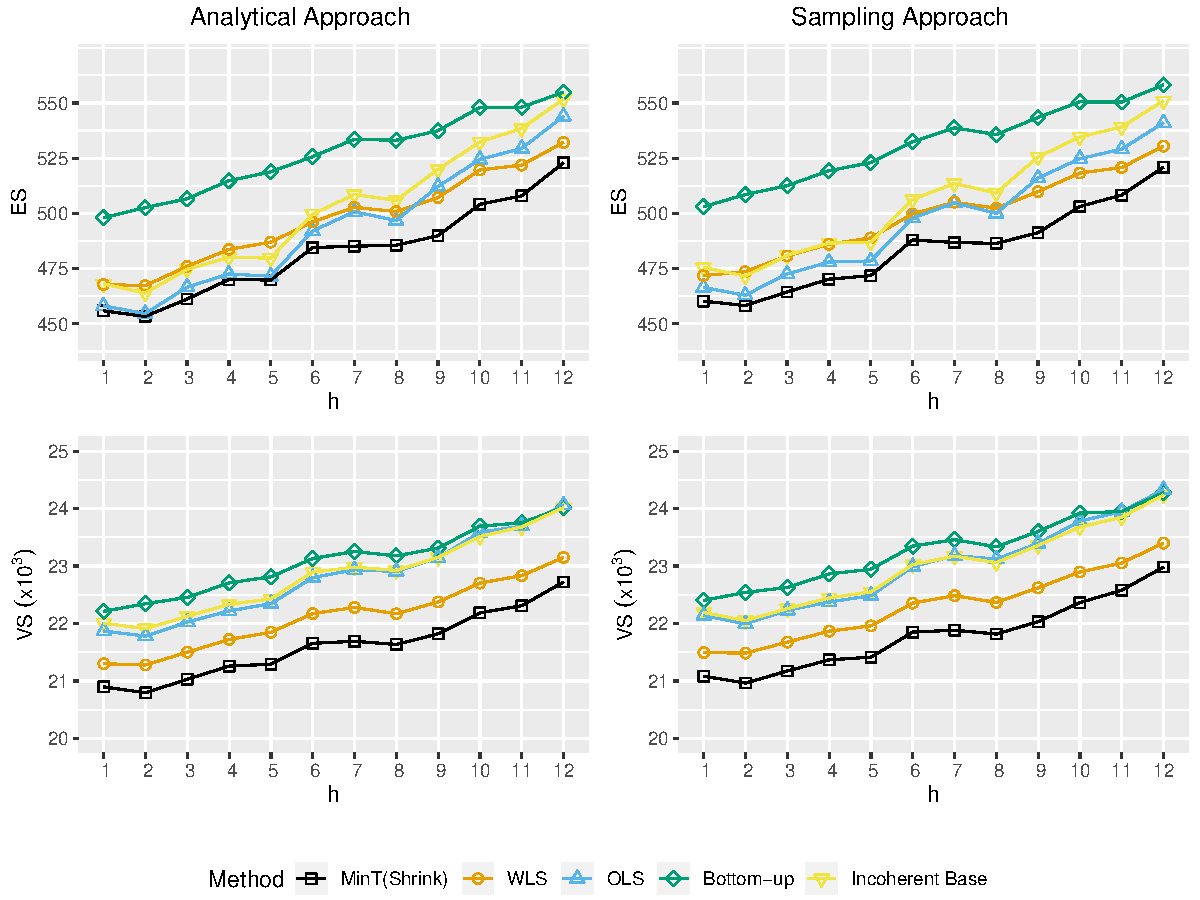
\includegraphics[width=.95\textwidth]{Empirical-results/Results-ARIMA/RawScore_Overall.pdf}
	\caption{Energy and variogram scores for multivariate predictive distributions across the entire hierarchy. A lower (higher) score indicates a more (less) accurate forecast. Results from the analytic approach assuming Gaussian incoherent base forecasts are presented on the left while results from the non-parametric approach are presented on the right.} \label{fig:Scores_Overall}
\end{figure}

As shown in Figure \ref{fig:Scores_Overall}, applying MinT(Shrink) for reconciliation of incoherent base forecasts generates the most accurate forecasts in all cases. As expected accuracy for all forecasts deteriorates as the forecast horizon increases. The skill scores presented in Figure \ref{fig:SkillScores_Overall} for the analytic solution show improvements upon the incoherent Gaussian base forecasts across the hierarchy as a whole. The improvements start at 2.5\% for $h=1$ and increase to above 5\% for $h\ge 9$ for the energy score and are consistently above 5\% for the variogram score. Note that in all cases the bottom-up forecasts are always inferior to the incoherent base forecasts. This comes to no surprise reflecting upon the fact that the bottom-level series are the noisiest and most challenging to forecast and information is lost when levels above are not considered as with a reconciliation approach.

\begin{figure}
	\centering
	\small
    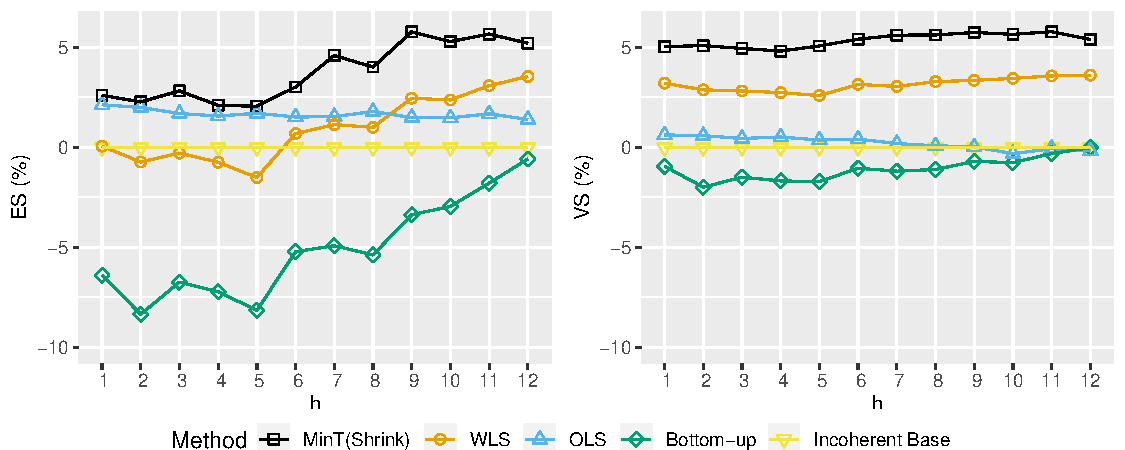
\includegraphics[width=.95\textwidth]{Empirical-results/Results-ARIMA/SkillScore_Overall.pdf}
	\caption{Skill scores (\%) relative to incoherent base forecasts, across the entire Australian tourism hierarchy based on energy score (on the left) and variogram score (on the right). A higher (lower) score indicates a gain (loss) in forecast accuracy relative to the incoherent base forecasts. The results are for the analytic solution assuming Gaussian incoherent base forecasts.} \label{fig:SkillScores_Overall}
\end{figure}

Figure \ref{fig:ES-SS-Levels} shows skill scores (\%) for the Gaussian analytic approach, relative to the incoherent base forecasts across each level of the Australia tourism hierarchy (please see Figure \ref{fig:ES-Levels} in Appendix \ref{app:AustralianData} for the raw scores). The top-panel presents the results for the aggregate level based on the CRPS, the univariate equivalent to the Energy score. For the levels below skill scores based on both the energy and variogram scores are presented.

Based on both scoring rules MinT(Shrink) improves upon the incoherent base forecasts at all levels and all forecast horizons (the only exception being forecast horizons 4 and 5 at the top-level for which a marginal loss is shown). The improvements for the top-level seem to be higher for the longer forecast horizons, increasing to 5\% or more for $h\ge7$. For the levels below the improvements seem to be more homogenous across the forecast horizons. Based on the energy score improvements are around 3\%, 4\% and 2\% for States, Zones and Regions respectively. These are considerably higher based on the variogram score for which gains around 10\%, 7\% and 3\% are shown. \textcolor{red}{We could comment on the bottom-up and the OLS results but I am not sure it is worth it.}

\begin{figure}
	\centering
	\small
	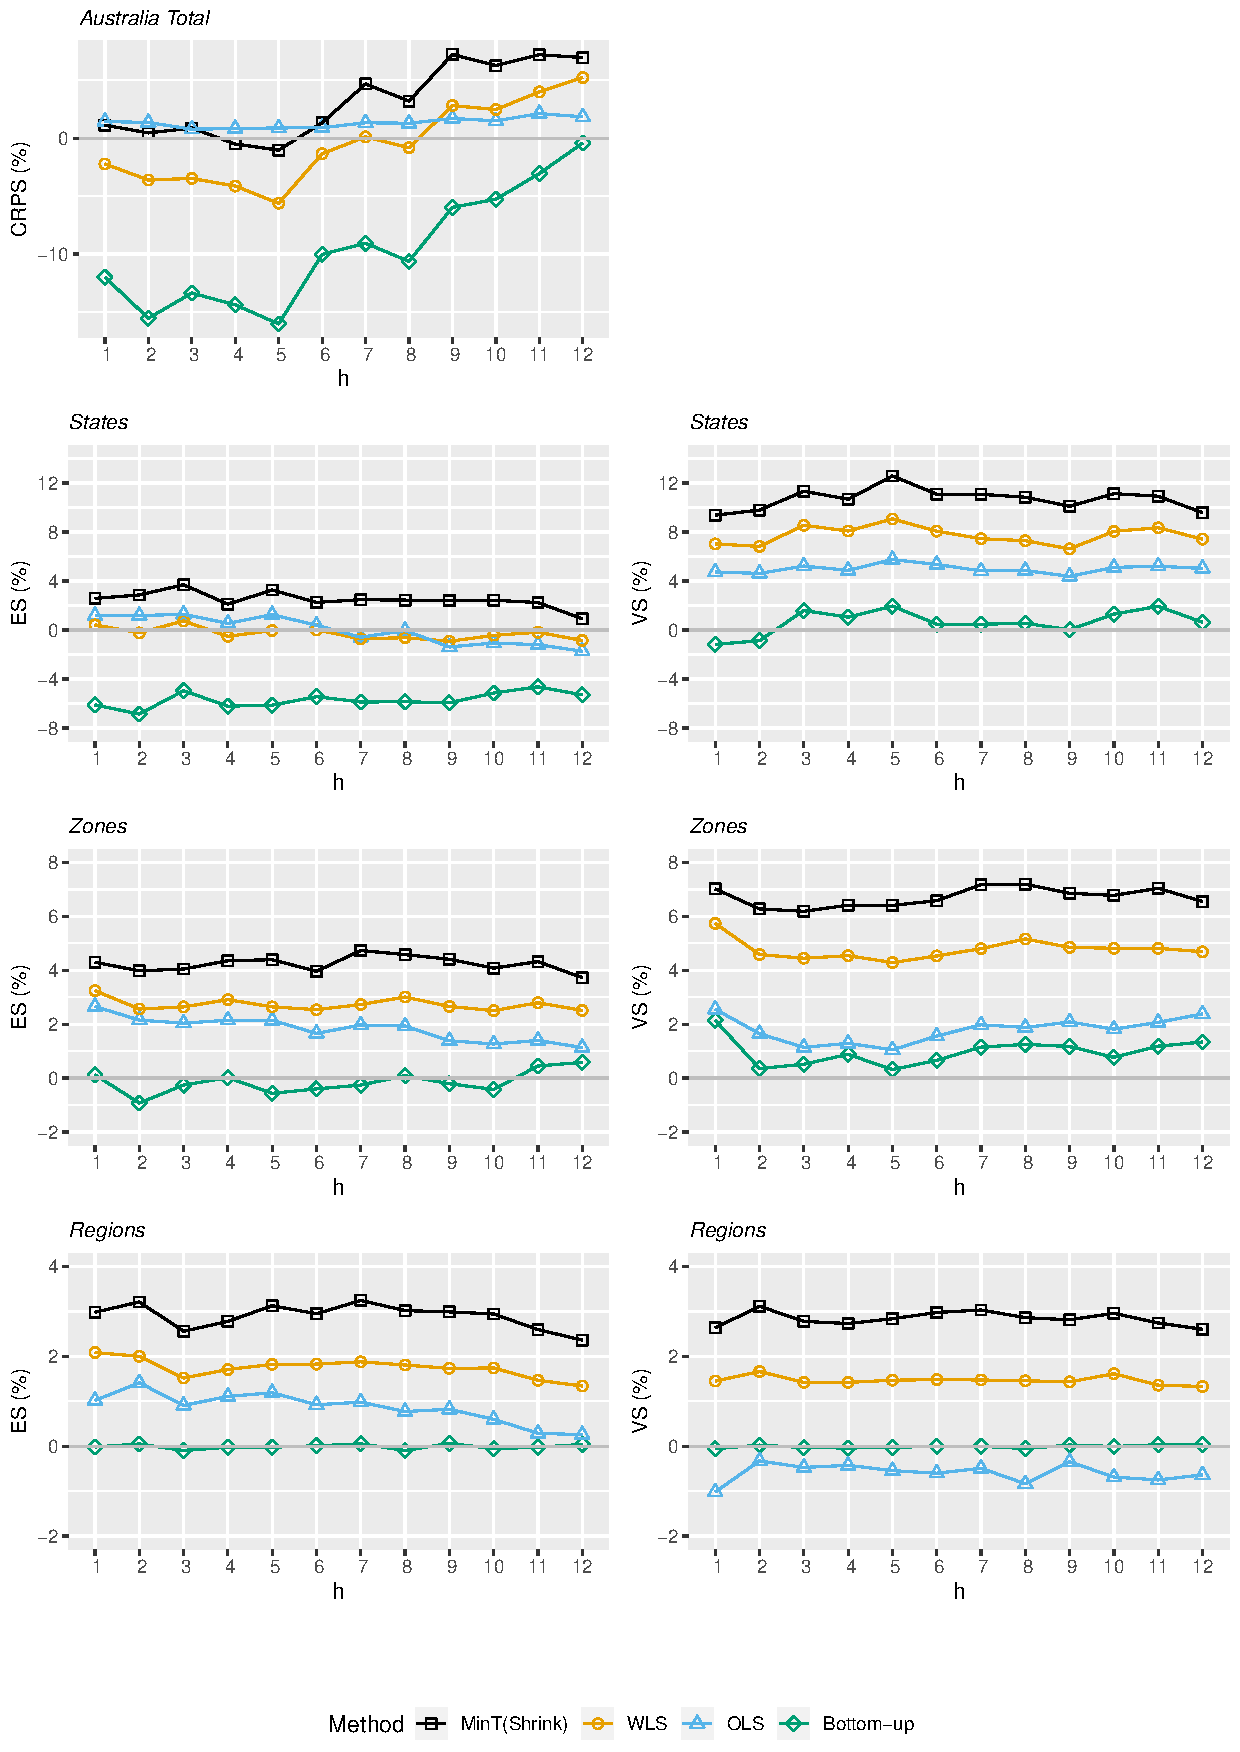
\includegraphics[width= 0.85\textwidth, height= 0.85\textheight]{Empirical-results/Results-ARIMA/SkillScore_Gauss_Levels.pdf}
	\caption{Skill scores (\%) relative to incoherent base forecasts, for the CRPS for the top-level and energy and variogram scores for the levels below for the Australia tourism hierarchy. A higher (lower) score indicates a gain (loss) in forecast accuracy relative to the incoherent base forecasts. All results are for the analytic solution assuming Gaussian incoherent base forecasts.} \label{fig:ES-SS-Levels}
\end{figure}


\section{Conclusions}\label{sec:conclusion}

Although hierarchical point forecasting is well studied in the literature, there has been a relative lack of attention given to the probabilistic setting. We fill this gap in the literature by providing a mathematically rigorous formulation of coherence and reconciliation for probabilistic forecasts.

The geometric interpretation of point forecast reconciliation can be extended to the probabilistic setting. We have also discussed strategies for evaluating probabilistic forecasts for hierarchical time series advocating the use of multivariate scoring rules on the full hierarchy, while establishing a key result that the log score is not proper with respect to incoherent forecasts.

We have shown that for elliptical distributions the true predictive density can be recovered by linear reconciliation and we have established conditions for when this is a projection. Although this projection cannot feasibly be obtained in practice, a projection similar to the MinT approach provides a good approximation in applications. This is supported by the results of a simulation study as well as the empirical application.

We have further proposed a novel non-parametric approach for obtaining coherent probabilistic forecasts for when the parametric densities are unavailable. Initially this method involves generating thousands of sample paths using bootstrapped forecast errors. Then each sample path is reconciled via projections. Using an extensive simulation setting we have shown that the MinT projection is at least as good as the optimal projection with respect to minimising Energy score. Further we have shown in an empirical application that reconciled probabilistic forecasts via MinT show gains in the forecast accuracy over incoherent and bottom-up forecasts.


In many ways this chapter sets up a substantial future research agenda. For example, having defined what amounts to an entire class of reconciliation methods for probabilistic forecasts it will be worthwhile investigating which specific projections are optimal. This is likely to depend on the specific scoring rule employed as well as the properties of the base forecasts. Another avenue worth investigating is to consider whether it is possible to recover the true predictive distribution for non-elliptical distributions via a non-linear function $g(.)$.

\newpage

\appendix

\section{Proof of Theorem~\ref{theo:bottomdens} and Theorem~\ref{theo:fulldens}} \label{app:Bottom&FullDens}

Consider the region $\mathcal{I}$ given by the Cartesian product of intervals $(l_1,u_1),(l_2,u_2),\ldots(l_m,u_m)$.  We derive the probability, under the reconciled measure, that the bottom-level series lie in $\mathcal{I}$, i.e. $\mbox{Pr}(\bm{l}\succ\bm{b}\succ\bm{u})$, where ${\bm l}=(l_1,l_2,\ldots,l_m)$, ${\bm u}=(u_1,u_2,\ldots,u_m)$ and $\succ$ denotes element-wise inequality between vectors.  The pre-image of $\mathcal{I}$ under $g$ can similarly be denoted as all points ${\bm y}$ satisfying $\bm{l}\succ\bm{G}\bm{y}\succ\bm{u}$.  Using Definition~\ref{def:reconprob},
\[
\mbox{Pr}(\bm{l}\succ\bm{b}\succ\bm{u})=\int\limits_{\bm{l}\succ\bm{G}\bm{y}\succ\bm{u}}\hat{f}(\bm{y})d{\bm y}\,,
\]
where $\hat{f}$ is the density of the base probabilistic forecast.  Now consider a change of variables to an $n$-dimensional vector ${\bm z}$ where $\bm{y}={\bm G^*}{\bm z}$. Recall, ${\bm G^*}=\left({\bm G^{-}}\,\vdots\,{\bm G_\perp}\right)$, ${\bm G^{-}}$ is a generalised inverse of $\bm{G}$ and ${\bm G_\perp}$ is an orthogonal complement of $\bm{G}$.  By the change of variables

\begin{align}
\mbox{Pr}(\bm{l}\succ\bm{b}\succ\bm{u})&=\int\limits_{\bm{l}\succ\bm{G}\bm{y}\succ\bm{u}}\hat{f}(\bm{y})d{\bm y}\nonumber\\
&=\int\limits_{\bm{l}\succ\bm{G}\bm{G}^*\bm{z}\succ\bm{u}}\hat{f}(\bm{G}^*\bm{z})|\bm{G}^*|d{\bm z}\nonumber\\
&=\int\limits_{\bm{l}\succ\bm{z}_1\succ\bm{u}}\hat{f}(\bm{G}^*\bm{z})|\bm{G}^*|d{\bm z}\nonumber\,,
\end{align}
where $\bm{z}_1$ denotes the first $m$ elements of $\bm z$.  Letting $\bm{a}$ denote the last $n-m$ elements of $\bm{z}$ the integral above can be written as
\[
\mbox{Pr}({\bm b}\in \mathcal{I})=\int\limits_{\bm{l}\succ\bm{z}_1\succ\bm{u}}\int\hat{f}(\bm{G}^{-}\bm{z}_1+\bm{G}_{\perp}\bm{a})|\bm{G}^*|d{\bm a}d{\bm z}_1\nonumber\\
\]
Replacing ${\bm z}_1$ with ${\bm b}$, it can be seen that the term inside the outer integral is a density for the bottom-level series. Therefore

\begin{equation}
\tilde{f}_{\bm{b}}(\bm{b})=\int\hat{f}(\bm{G}^{-}\bm{b}+\bm{G}_{\perp}\bm{a})|\bm{G}^*|d{\bm a}\,,
\label{eq:densb}
\end{equation}
is the density of ${\bm b}$. To obtain the density of the full hierarchy we first augment the density in Equation \eqref{eq:densb} by $n-m$ variables denoted $\bm{u}$

\begin{equation}
f(\bm{b},\bm{u})=\tilde{f}_b(\bm{b})\mathbb{1}\left\{\bm{u}=0\right\}\,,
\end{equation}
such that the density $f(\bm{b},\bm{u})$ is a density for $n$-dimensional vector that is degenerate across the dimensions corresponding to $\bm{u}$.  Using the change of variables,
\[
\bm{y}=\left(\bm{S}\,\vdots\,\bm{S}^-_{\perp}\right)\begin{pmatrix}\bm{b}\\\bm{u}
\end{pmatrix}\,,
\]
where $\bm{S}^-_{\perp}$ is a generalised inverse such that $\bm{S}'_{\perp}\bm{S}^-_{\perp}=\bm{I}$ and noting the inverse of $\left(\bm{S}\,\vdots\,\bm{S}_{\perp}\right)$ is given by
\[
\bm{S}^*:=\begin{pmatrix}\bm{S}^{-}\\\bm{S}'_{\perp}\end{pmatrix}\,,
\]
it can be seen that $\bm{b}=\bm{S}^-\bm{y}$ and $\bm{u}=\bm{S}'_\perp\bm{y}$.  Applying this change of variables yields the density
\[
\tilde{f}_{\bm{y}}(\bm{y})=|\bm{S}^*|\tilde{f}_{\bm b}(\bm{S}^-\bm{y})\mathbb{1}\left\{\bm{S}'_\perp\bm{y}=\bm{0}\right\}\,.
\]
Since $\bm{S}'_\perp$ is the orthogonal complement of $\bm{S}$ and since the columns of $\bm{S}$ span the coherent subspace, the statement $\bm{S}'_\perp\bm{y}=0$ is equivalent to the statement $\bm{y}\in\mathfrak{s}$.  As such, the reconciled density is given by
\[
\tilde{f}_{\bm{y}}(\bm{y})=|\bm{S}^*|\tilde{f}_b(\bm{S}^-\bm{y})\mathbb{1}\left\{\bm{y}\in\mathfrak{s}\right\}.
\]
\clearpage
\section{Proof of Theorem~\ref{theo:OptRecProj}}
\label{app:OptRecProj}

Let
\[
\hat{\bm{\Sigma}}=\bm{\Sigma}+{\bm D}=\bm{S}\bm{\Omega}{\bm{S}}'+{\bm D}\,.
\]
If reconciliation is carried out via a projection onto $\mathfrak{s}$, then $\bm{S}\bm{G}\bm{S}=\bm{S}$ and
\begin{align}
\tilde{\bm{\Sigma}}&=\bm{S}\bm{G}\hat{\bm{\Sigma}}\bm{G}'\bm{S}'\nonumber\\
&\bm{S}\bm{G}\bm{S}\bm{\Omega}\bm{S}'\bm{G}'{\bm{S}}'+\bm{S}\bm{G}{\bm D}\bm{G}'\bm{S}'\nonumber\\
&\bm{S}\bm{\Omega}{\bm{S}}'+\bm{S}\bm{G}{\bm D}\bm{G}'\bm{S}'\nonumber\\
&\bm{\Sigma}+\bm{S}\bm{G}{\bm D}\bm{G}'\bm{S}'\nonumber\,.
\end{align}
Therefore to recover the true predictive using a projection, some ${\bm G}_0$ must be found such that ${\bm G}_0{\bm D}=\bm{0}$. Let the eigenvalue decomposition of $\bm {D}$ be given by  ${\bm R}{\bm \Lambda}{\bm R}'$ , where ${\bm R}$ is an $n\times q$ matrix with $q=\textrm{rank}({\bm{D}})$ and ${\bm\Lambda}$ is an $q\times q$ diagonal matrix containing non-zero eigenvalues of ${\bm D}$.  By the rank nullity theorem, $\bm{R}$ will have an orthogonal complement $\bm{R}_{\perp}$ of dimension $n\times (n-q)$.  If $q=n-m$ then the number of columns of $\bm{R}_{\perp}$ is $m$ and ${\bm G}_0$ can be formed as the $m\times n$ matrix $(\bm{R}_{\perp}'\bm{S})^{-1}\bm{R}_{\perp}'$.  If $q<n-m$ the number of columns of $\bm{R}_{\perp}$ is greater than $m$, and any $m$ columns of $\bm{R}_{\perp}$ can be used to form ${\bm G}_0$ in a similar fashion.  However when $q>n-m$, the number of columns of $\bm{R}_{\perp}$ is less than $m$ and no such $m\times n$ matrix ${\bm G}_0$ can be formed.  Therefore the true predictive can only be recovered via a projection when $\textrm{rank}({\bm D})\leq n-m$.

With respect to the location, if $\bm{SG}$ is a projection then reconciled forecasts will be unbiased as long as the base forecasts are also unbiased.  When base forecasts are biased they can be bias corrected before reconciliation as described by \cite{PanEtAl2019HF} in the point forecasting setting.

\clearpage
\section{Proof of Theorem~\ref{theo:logS_improp}}\label{app:logS_improp}

The proof relies on the following change of variables,
\[
\bm{y}=\left(\bm{S}\,\vdots\,\bm{S_\perp}\right)\begin{pmatrix}\bm{b}\\\bm{u}\end{pmatrix}.
\]
Also recall from the proof of Theorem~\ref{theo:fulldens} that $\bm{S}^*=\left(\bm{S}\,\vdots\,\bm{S_\perp}\right)^{-1}$

Let the density of the true predictive $f(\bm{y})$ after a change of variables, be given by $|\bm{S^*}|^{-1}f_{\bm b}(\bm{b})\mathbb{1}\left\{\bm{u}=\bm{0}\right\}$.  To prove that the log score is improper we construct an incoherent base density $\hat{f}$ such that $E_f\left[LS\left(\hat{f},\bm{y}\right)\right]<E_f\left[LS\left(f,\bm{y}\right)\right]$. This incoherent density is constructed, so that after the same change of variables it can be written as $|\bm{S^*}|^{-1}\hat{f}_{\bm b}(\bm{b})\hat{f}_{\bm{u}}(\bm{u})$. We require $\hat{f}_{\bm u}(\bm{0})>1$, i.e., ${\bm u}$ is highly concentrated around $\bm{0}$ but still non-degenerate. An example is an independent normal with mean 0 and variances less than $(2\pi)^{-1}$. Now, let $\bm{y}^*$ be a realisation from $f$. Let the first $m$ elements of $\bm{S}^*\bm{y}^*$ be $\bm{b^*}$, and the remaining elements be ${\bm u}^*$.  The log score for $f$ is thus,	
\begin{align}
LS\left(f,\bm{y}^*\right) &= -\log f(\bm{y}^*) \nonumber\\
&=-\log|\bm{S^*}|-\log f_{\bm{b}}\left(\bm{b}^*\right)-\log\left(\mathbb{1}\left\{\bm{u}^*=\bm{0}\right\}\right)\label{eq:diraccancel}\\
&=-\log|\bm{S^*}|-\log f_{\bm{b}}\left(\bm{b}^*\right),\nonumber
\end{align}
where the third term in Equation~\ref{eq:diraccancel} is equal to zero since the fact that $\bm{y}^*\in\mathfrak{s}$ implies that $\bm{u}^*=\bm{0}$.  The log score for $\hat{f}$ is
\[
LS\left(\hat{f},\bm{y}^*\right) = -\log|\bm{S^*}|-\log f_{\bm{b}}(\bm{b}^*)- \log f_{\bm u}(\bm{0})\,.
\]
Since $f_{\bm u}(\bm{0})>1$ by construction, $-\log f_{\bm u}(\bm{0})<0$, therefore
\[
LS\left(\hat{f},\bm{y}^*\right) <-\log|\bm{S^*}|-\log f_{\bm b}(\bm{b}^*)=LS\left(f,\bm{y}^*\right)
\]
Since this holds for any possible realisation, it will also hold after taking expectations (by the monotonicity of expectations).  Thus $\hat{f}$ violates the condition for a proper scoring rule.

\clearpage
\section{Data generating process} \label{app:DGP}

To ensure that bottom level series are noisier than top level series (a feature often observed empirically), noise is added to the bottom level series in the following manner
\begin{align*}
y_{AA,t} &= w_{AA,t} + u_t - 0.5v_t,\\
y_{AB,t} &= w_{AB,t} - u_t - 0.5v_t,\\
y_{BA,t} &= w_{BA,t} + u_t + 0.5v_t,\\
y_{BB,t} &= w_{BB,t} - u_t + 0.5v_t,
\end{align*}
where $w_{AA,t},w_{AB,t},w_{BA,t},w_{BB,t}$ generated from ARIMA processes as described in Section\ref{sec:dgp} with innovations $\varepsilon_{AA,t},\varepsilon_{AB,t},\varepsilon_{BA,t},\varepsilon_{BB,t}$. Aggregating the bottom-level series gives the following for the aggregated levels,
\begin{align*}
y_{A,t} &= w_{AA,t} + w_{AB,t} - v_t,\\
y_{B,t} &= w_{BA,t} + w_{BB,t} + v_t,\\
y_{Tot,t} &= w_{AA,t} + w_{AB,t} + w_{BA,t} + w_{BB,t}.
\end{align*}


For the Gaussian DGP, $u_t \sim \mathcal{N}(0,\sigma^2_u)$ and $v_t \sim \mathcal{N}(0,\sigma^2_v)$ and the errors driving the bottom-level ARIMA processes are jointly generated from a Normal distribution while . More specifically, $\{\varepsilon_{AA,t},\varepsilon_{AB,t},\varepsilon_{BA,t},\varepsilon_{BB,t}\} \overset{iid}{\sim} \mathcal{N}(\bm{0}, \bm{\Sigma})~\forall t$.  We follow \cite{WicEtAl2019} and set
\begin{equation*}\label{eq:SigmaGaussian}
\bm{\Sigma} =
\begin{pmatrix}
5.0 & 3.1 & 0.6 & 0.4 \\
3.1 & 4.0 & 0.9 & 1.4 \\
0.6 & 0.9 & 2.0 & 1.8 \\
0.4 & 1.4 & 1.8 & 3.0 \\
\end{pmatrix}
\end{equation*} and $\sigma^2_u=28$ and $\sigma^2_v=22$. This ensures that the following inequalities are satisfied,
\begin{align*}
\var(\varepsilon_{AA,t} + \varepsilon_{AB,t} + \varepsilon_{BA,t} + \varepsilon_{BB,t})
\le \var(\varepsilon_{AA,t}+\varepsilon_{AB,t}-v_t)
\le \var(\varepsilon_{AA,t}+u_t-0.5v_t),\\
\var(\varepsilon_{AA,t} + \varepsilon_{AB,t} + \varepsilon_{BA,t} + \varepsilon_{BB,t})
\le \var(\varepsilon_{AA,t}+\varepsilon_{AB,t}-v_t)
\le \var(\varepsilon_{AB,t}-u_t-0.5v_t),\\
\var(\varepsilon_{AA,t} + \varepsilon_{AB,t} + \varepsilon_{BA,t} + \varepsilon_{BB,t})
\le \var(\varepsilon_{BA,t}+\varepsilon_{BB,t}+v_t)
\le \var(\varepsilon_{BA,t}+u_t+0.5v_t),\\
\var(\varepsilon_{AA,t} + \varepsilon_{AB,t} + \varepsilon_{BA,t} + \varepsilon_{BB,t})
\le \var(\varepsilon_{BA,t}+\varepsilon_{BB,t}+v_t)
\le \var(\varepsilon_{BB,t}-u_t+0.5v_t).\\
\end{align*}

For the non-Gaussian case, errors are generated from a Gumbel copula with Beta margins as described in Section~\ref{sec:dgp}. Rather than add Gaussian noise, we simulate $u_t$ and $v_t$ from skew t distributions using the package \cite.  The scale, skew and degrees of freedom parameters are chosen as 0.5,1.5 and 4 and 0.9,2 and 8 for $u_t$ and $v_t$ respectively.  Monte Carlo simulations show that these values satisfy the inequalities described above.

\clearpage
\section{Simulation results from parametric solution for marginal forecast distributions for $h=2$ and $h=3$}\label{app:AnalysticalSolMargins}

\begin{table}[H]
	\caption{Comparison of incoherent vs coherent forecasts based on the univariate forecast distribution of each series. Each entry represents the percentage skill score with reference to the incoherent forecasts based on ``CRPS" and ``LS". These entries show the percentage increase in score for different forecasting methods relative to the incoherent forecasts for $h=2$ step-ahead forecast. Results from the Gaussian DGP are presented in the top panel whereas the results from the non-Gaussian DGP are presented in the bottom panel}\label{tab:SimAnalyticalUni_h2}
	\centering
	\resizebox{\linewidth}{!}{
		\begin{tabular}{lcccccccccccccc}
			\toprule
			\multicolumn{1}{c}{ } & \multicolumn{7}{c}{Gaussian} & \multicolumn{7}{c}{Non-Gaussian}\\
			\cmidrule(lr){2-8} \cmidrule(lr){9-15}
			Series & Tot & A & B & AA & AB & BA & BB & Tot & A & B & AA & AB & BA & BB \\
			\toprule
			\multicolumn{15}{c}{Log Score (\%)}\\
			\toprule
			Base & 0.00 & 0.00 & 0.00 & 0.00 & 0.00 & 0.00 & 0.00 & 0.00 & 0.00 & 0.00 & 0.00 & 0.00 & 0.00 & 0.00\\
			Bottom up & \textbf{9.87} & -0.72 & -4.28 & 0.00 & 0.00 & -10.02 & \textbf{18.99} & -8.05 & -0.30 & -3.12 & 0.00 & 0.00 & -1.46 & -11.80\\
			OLS & -22.52 & 1.31 & 0.50 & 1.81 & 0.25 & -6.72 & 18.12 & 30.16 & 0.20 & 3.28 & -1.53 & 4.33 & 0.18 & -10.70\\
			WLS & -27.45 & -13.81 & 26.50 & 2.41 & 0.57 & -6.17 & 5.10 & 12.65 & \textbf{7.09} & -6.06 & -1.55 & 4.11 & 0.71 & -1.67\\
			MinT(Sample) & -0.28 & 2.65 & 0.57 & \textbf{3.51} & \textbf{1.80} & -5.36 & 18.86 & -0.02 & 0.43 & \textbf{6.80}& \textbf{0.64} & 4.66 & \textbf{2.44} & -9.36\\
			MinT(Shrink) & -0.29 & 2.60 & 0.56 & 3.37 & 1.72 & -5.34 & 18.90 & -0.06 & 0.42 & 6.79 & -1.50 & \textbf{4.67} & 2.26 & -9.46\\
			Optimal & -12.70 & \textbf{5.42} & \textbf{26.71} & 2.86 & 0.52 & -6.42 & 17.11 & \textbf{34.04} & -2.98 & -7.45 & -6.28 & -0.19 & -2.31 & -14.48\\	
			\toprule
			\multicolumn{15}{c}{CRPS (\%)}\\
			\toprule
			Base & 0.00 & 0.00 & 0.00 & 0.00 & 0.00 & 0.00 & 0.00 & 0.00 & 0.00 & 0.00 & 0.00 & 0.00 & 0.00 & 0.00\\
			Bottom up & -45.40 & -5.11 & -16.82 & 0.02 & -0.05 & -37.16 & 46.65 & -185.36 & -0.54 & -8.18 & 0.08 & -0.03 & -3.54 & -35.55\\
			OLS & -14.62 & 6.88 & 1.64 & 7.06 & 0.78 & -23.24 & 45.12 & 61.90 & 0.64 & 8.48 & -4.32 & 11.30 & 1.10 & -31.86\\
			WLS & -10.18 & -41.19 & 23.92 & 8.75 & 1.83 & -21.19 & 14.60 & 70.13 & \textbf{17.33} & -171.66 & -4.30 & 10.76 & 2.52 & -6.06\\
			MinT(Sample) & -0.13 & \textbf{12.14} & 2.13 & 11.19 & \textbf{6.18} & -17.67 & 46.49 & 0.26 & 1.29 & 16.54 & \textbf{1.60} & 11.95 & \textbf{6.76} & -27.69\\
			MinT(Shrink) & -0.08 & 12.03 & 2.05 & \textbf{11.62} & 5.74 & -17.91 & \textbf{46.64} & 0.32 & 1.44 & \textbf{16.71} & -4.15 & \textbf{12.14} & 6.54 & -27.79\\
			Optimal & -10.80 & 10.78 & \textbf{22.61} & 7.57 & -0.96 & -25.69 & 41.91 & \textbf{71.52} & -8.89 & -184.63 & -18.29 & -1.88 & -7.13 & -44.68\\
			\bottomrule
		\end{tabular}
	}
\end{table}

\begin{table}[H]
	\caption{Comparison of incoherent vs coherent forecasts based on the univariate forecast distribution of each series. Each entry represents the percentage skill score with reference to the incoherent forecasts based on ``CRPS" and ``LS". These entries show the percentage increase in score for different forecasting methods relative to the incoherent forecasts for $h=3$ step-ahead forecast. Results from the Gaussian DGP are presented in the top panel whereas the results from the non-Gaussian DGP are presented in the bottom panel}\label{tab:SimAnalyticalUni_h3}
	\centering
	\resizebox{\linewidth}{!}{
		\begin{tabular}{lcccccccccccccc}
			\toprule
			\multicolumn{1}{c}{ } & \multicolumn{7}{c}{Gaussian} & \multicolumn{7}{c}{Non-Gaussian}\\
			\cmidrule(lr){2-8} \cmidrule(lr){9-15}
			Series & Tot & A & B & AA & AB & BA & BB & Tot & A & B & AA & AB & BA & BB \\
			\toprule
			\multicolumn{15}{c}{Log Score (\%)}\\
			\toprule
			Base & 0.00 & 0.00 & 0.00 & 0.00 & 0.00 & 0.00 & 0.00 & 0.00 & 0.00 & 0.00 & 	0.00 & 0.00 & 0.00 & 0.00\\
			Bottom up & 34.32 & 1.21 & -3.97 & 0.00 & 0.00 & -14.82 & 29.16 & 56.40 & -0.15 & -2.89 & 0.00 & 0.00 & -1.73 & -11.81\\
			OLS & -67.52 & -0.68 & 0.48 & 0.27 & -0.27 & -10.97 & 28.06 & -5.91 & 0.47 & 2.87 & -1.78 & 5.14 & 0.07 & -10.68\\
			WLS & -85.70 & -26.29 & 50.39 & 0.68 & 0.12 & -10.26 & 10.40 & -129.42 & 10.02 & 57.99 & -1.71 & 4.84 & 0.75 & 1.18\\
			MinT(Sample) & -0.40 & -1.26 & 0.45 & 2.29 & 1.61 & -9.34 & 28.94 & -0.09 & 0.65 & 5.79 & 0.75 & 5.58 & 2.48 & -9.97\\
			MinT(Shrink) & -0.42 & -1.32 & 0.46 & 1.39 & 1.50 & -9.27 & 28.99 & -0.16 & 0.63 & 5.77 & -1.74 & 5.60 & 2.34 & -9.93\\
			Optimal & -24.58 & 10.50 & 51.73 & 2.73 & 3.03 & -8.64 & 27.28 & -12.25 & -2.65 & 57.70 & -7.44 & 0.17 & -2.67 & -15.72\\
			\toprule
			\multicolumn{15}{c}{CRPS (\%)}\\
			\toprule
			Base & 0.00 & 0.00 & 0.00 & 0.00 & 0.00 & 0.00 & 0.00 & 0.00 & 0.00 & 0.00 & 0.00 & 0.00 & 0.00 & 0.00\\
			Bottom up & -22.10 & -3.52 & -16.10 & -0.04 & -0.09 & -53.20 & 58.23 & -80.43 & -0.35 & -8.48 & -0.17 & -0.05 & -4.20 & -36.03\\
			OLS & -47.20 & 4.67 & 2.04 & 2.52 & 0.48 & -36.36 & 56.33 & 44.08 & 1.46 & 7.70 & -4.75 & 13.40 & 0.90 & -31.65\\
			WLS & -44.96 & -60.44 & 42.85 & 3.92 & 1.71 & -33.62 & 25.60 & 46.73 & 22.77 & -66.37 & -4.90 & 12.58 & 2.58 & -0.12\\
			MinT(Sample) & 0.02 & 7.99 & 2.21 & 9.03 & 6.23 & -29.83 & 57.85 & 0.21 & 1.88 & 14.24 & 1.88 & 14.20 & 6.81 & -29.36\\
			MinT(Shrink) & -0.03 & 7.89 & 2.34 & 6.61 & 6.05 & -29.59 & 57.94 & 0.15 & 1.75 & 14.18 & -4.92 & 14.34 & 6.61 & -29.31\\
			Optimal & -30.12 & 13.11 & 42.74 & 4.33 & 5.29 & -34.52 & 54.09 & 54.69 & -8.71 & -75.04 & -22.55 & -0.69 & -8.13 & -50.60\\
			\bottomrule
		\end{tabular}
	}
\end{table}


%\section{Application}
%
%\subsection{Results from ETS base forecasts}
%
%\begin{figure}[!hbt]
%	\centering
%	\small
%%	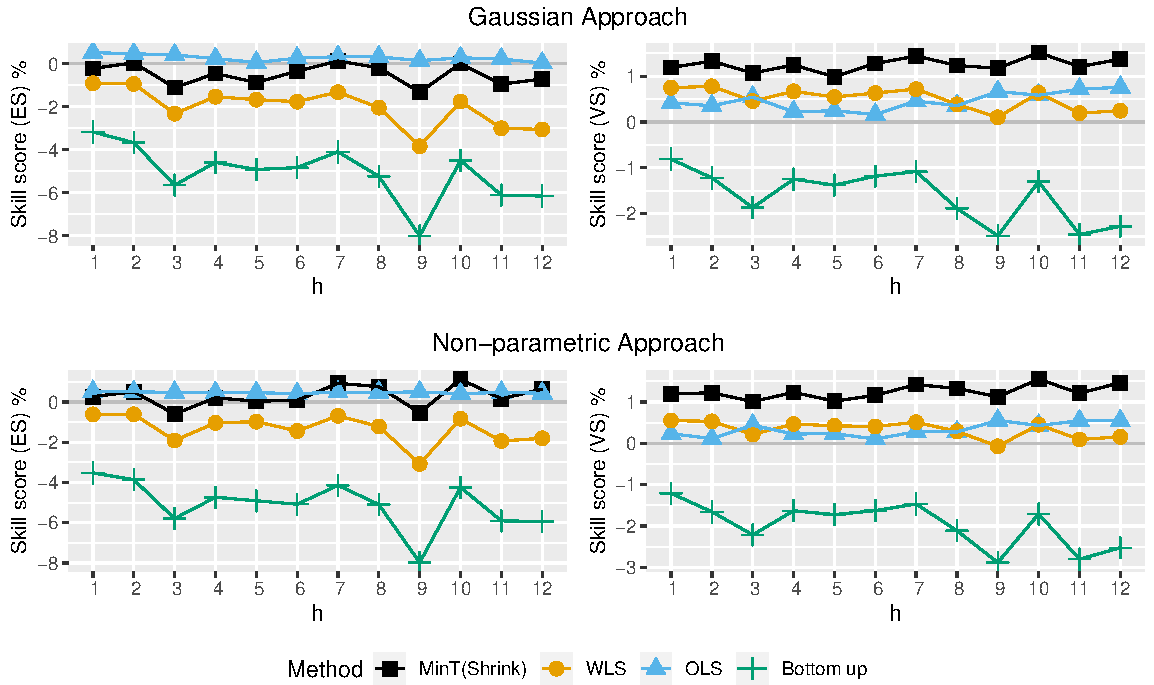
\includegraphics[width= .95\textwidth]{Empirical-results/AllTS_MultiVScores_ETS.pdf}
%	\caption{Skill scores with reference to ETS base forecasts for multivariate predictive distribution of the whole hierarchy from different reconciliation methods are presented. Top panel shows the results from Gaussian approach and the bottom panel shows the results from non-parametric approach. Left and right panels shows the skill scores based on energy score and variogram score respectively.}\label{fig:EmpResults_AllTS_ETS}
%\end{figure}
%
%\begin{figure}[!hbt]
%	\centering
%	\small
%%	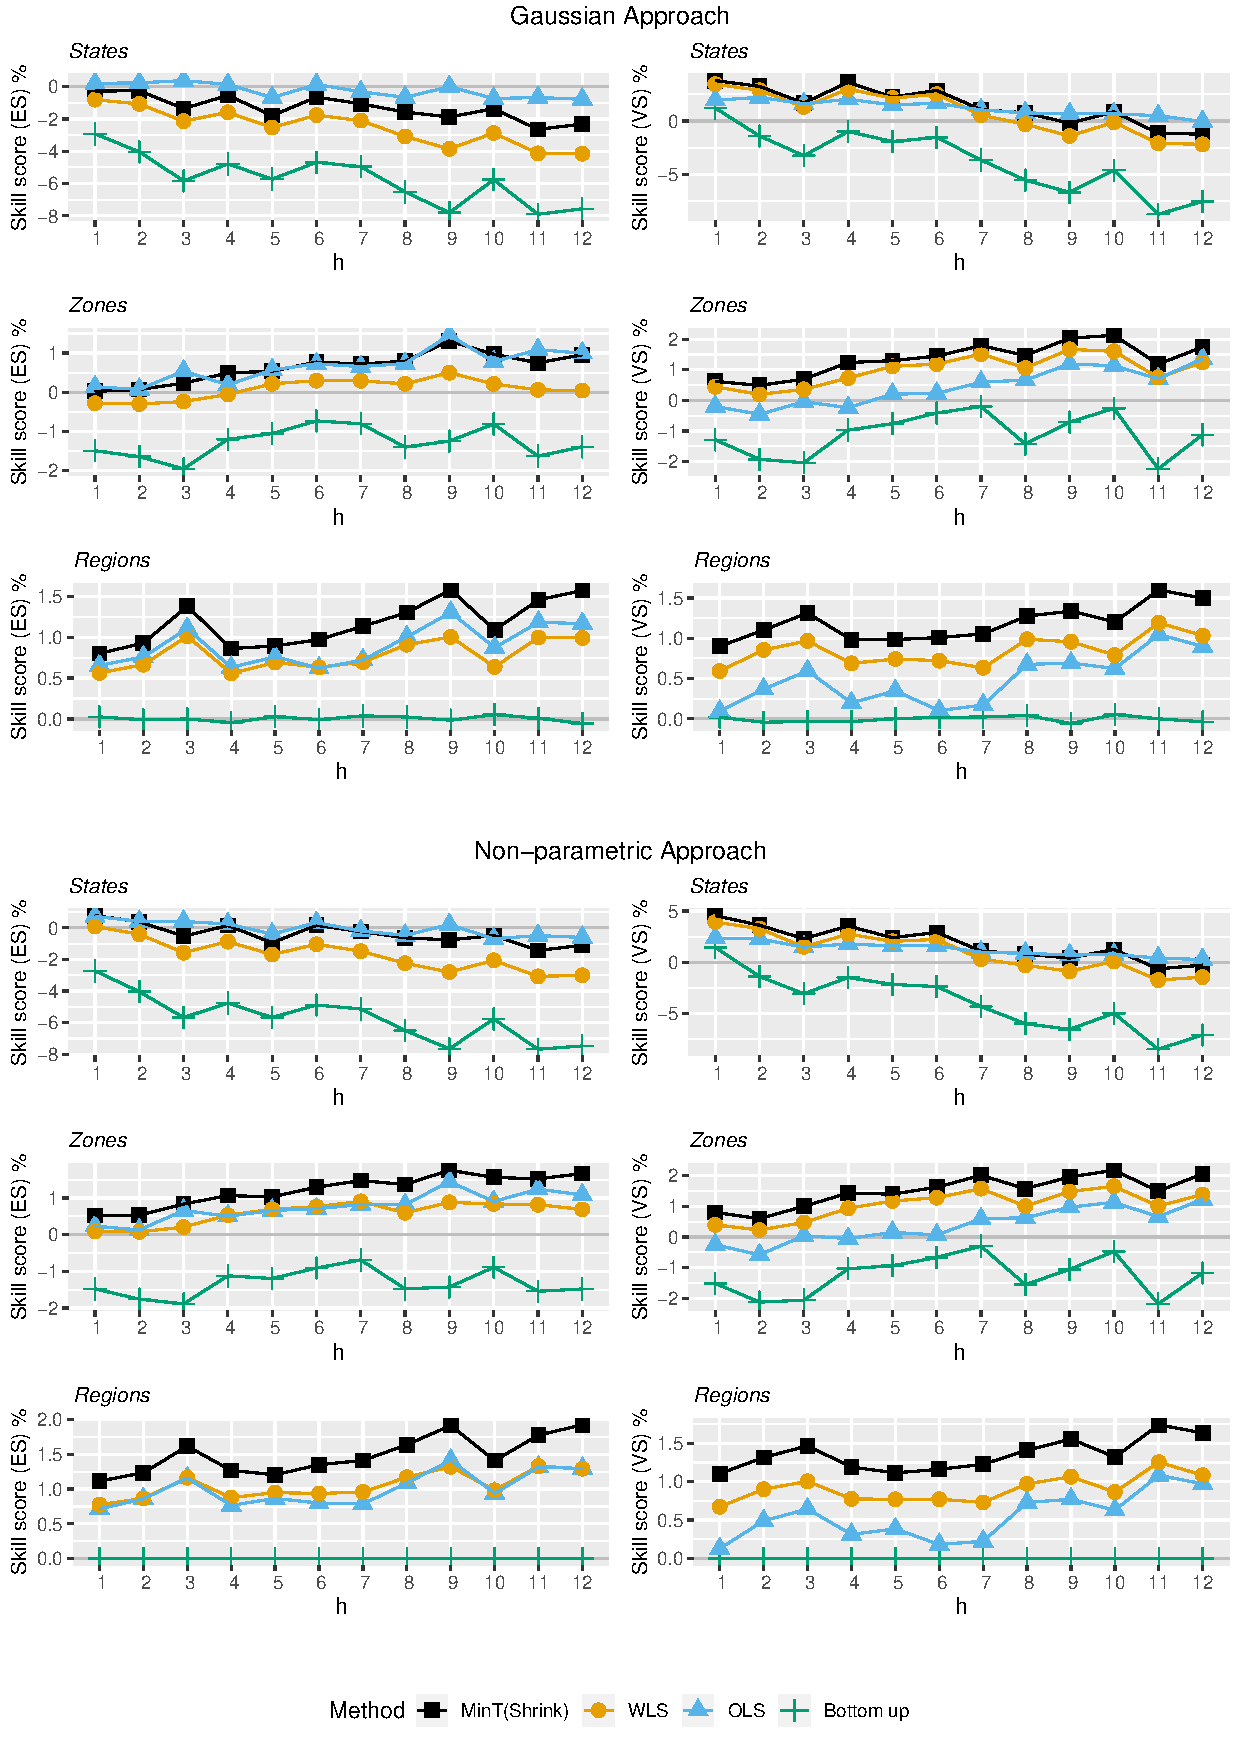
\includegraphics[width= 0.8\textwidth, height= 0.85\textheight]{Empirical-results/Levels_MultiVScores_ETS.pdf}
%	\caption{Skill score (with reference to ETS base forecasts) for multivariate probabilistic forecasts of different levels of the hierarchy are presented. Results from Gaussian approach are presented in the top three panels and results from the non-parametric approach are presented in the bottom three panels.}\label{fig:EmpResults_Levels_ETS}
%\end{figure}
%
%\begin{figure}[!hbt]
%	\centering
%	\small
%%	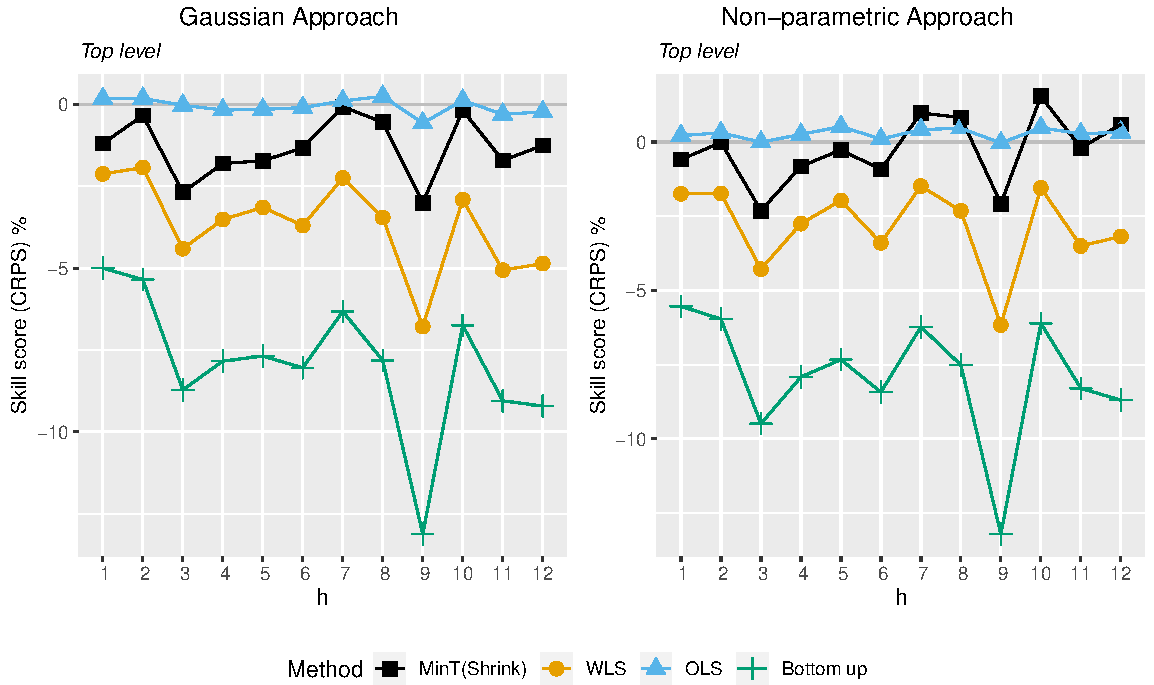
\includegraphics[width= \textwidth]{Empirical-results/UniVScore_TopLevel_ETS.pdf}
%	\caption{Skill score based on CRPS (with reference to the ETS base forecasts) for univariate probabilistic forecasts for the Total (top level) overnight trips are presented. Left panel shows the results from Gaussian approach and right panel shows the results from non-parametric approach. }\label{fig:EmpResults_TopLevel_ETS}
%\end{figure}
\clearpage
\section{Application}

\subsection{Results from ETS base forecasts}

\begin{figure}[!hbt]
	\centering
	\small
%	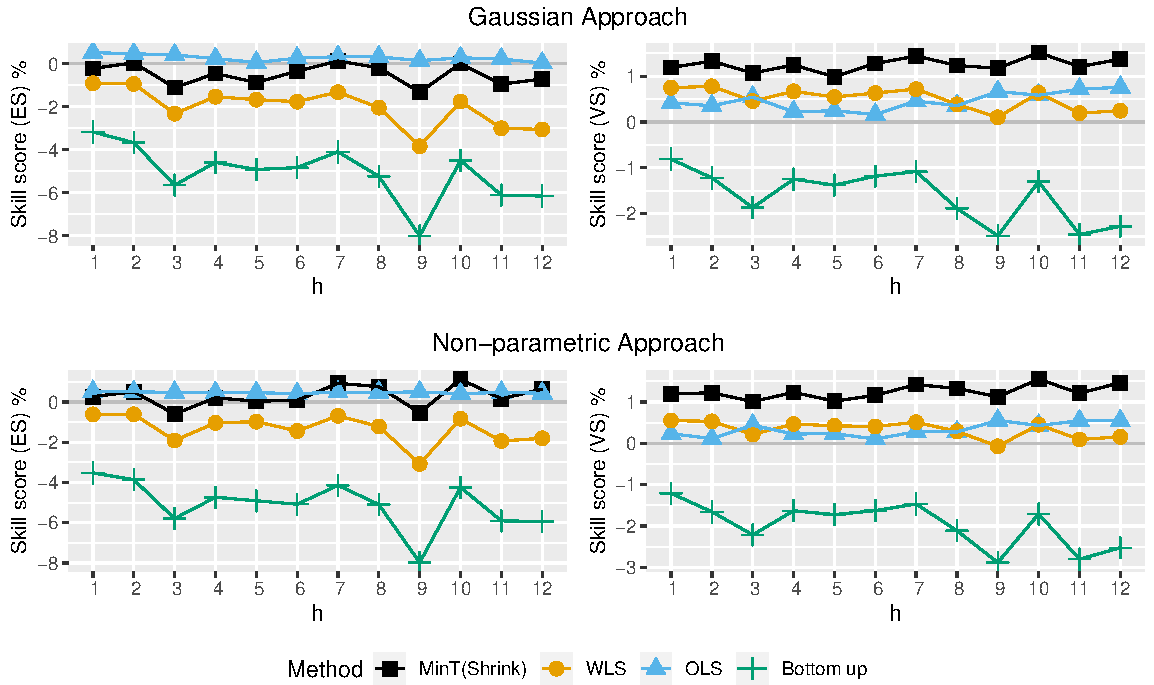
\includegraphics[width= .95\textwidth]{Empirical-results/AllTS_MultiVScores_ETS.pdf}
	\caption{Skill scores with reference to ETS base forecasts for multivariate predictive distribution of the whole hierarchy from different reconciliation methods are presented. Top panel shows the results from Gaussian approach and the bottom panel shows the results from non-parametric approach. Left and right panels shows the skill scores based on energy score and variogram score respectively.}\label{fig:EmpResults_AllTS_ETS}
\end{figure}

\begin{figure}[!hbt]
	\centering
	\small
%	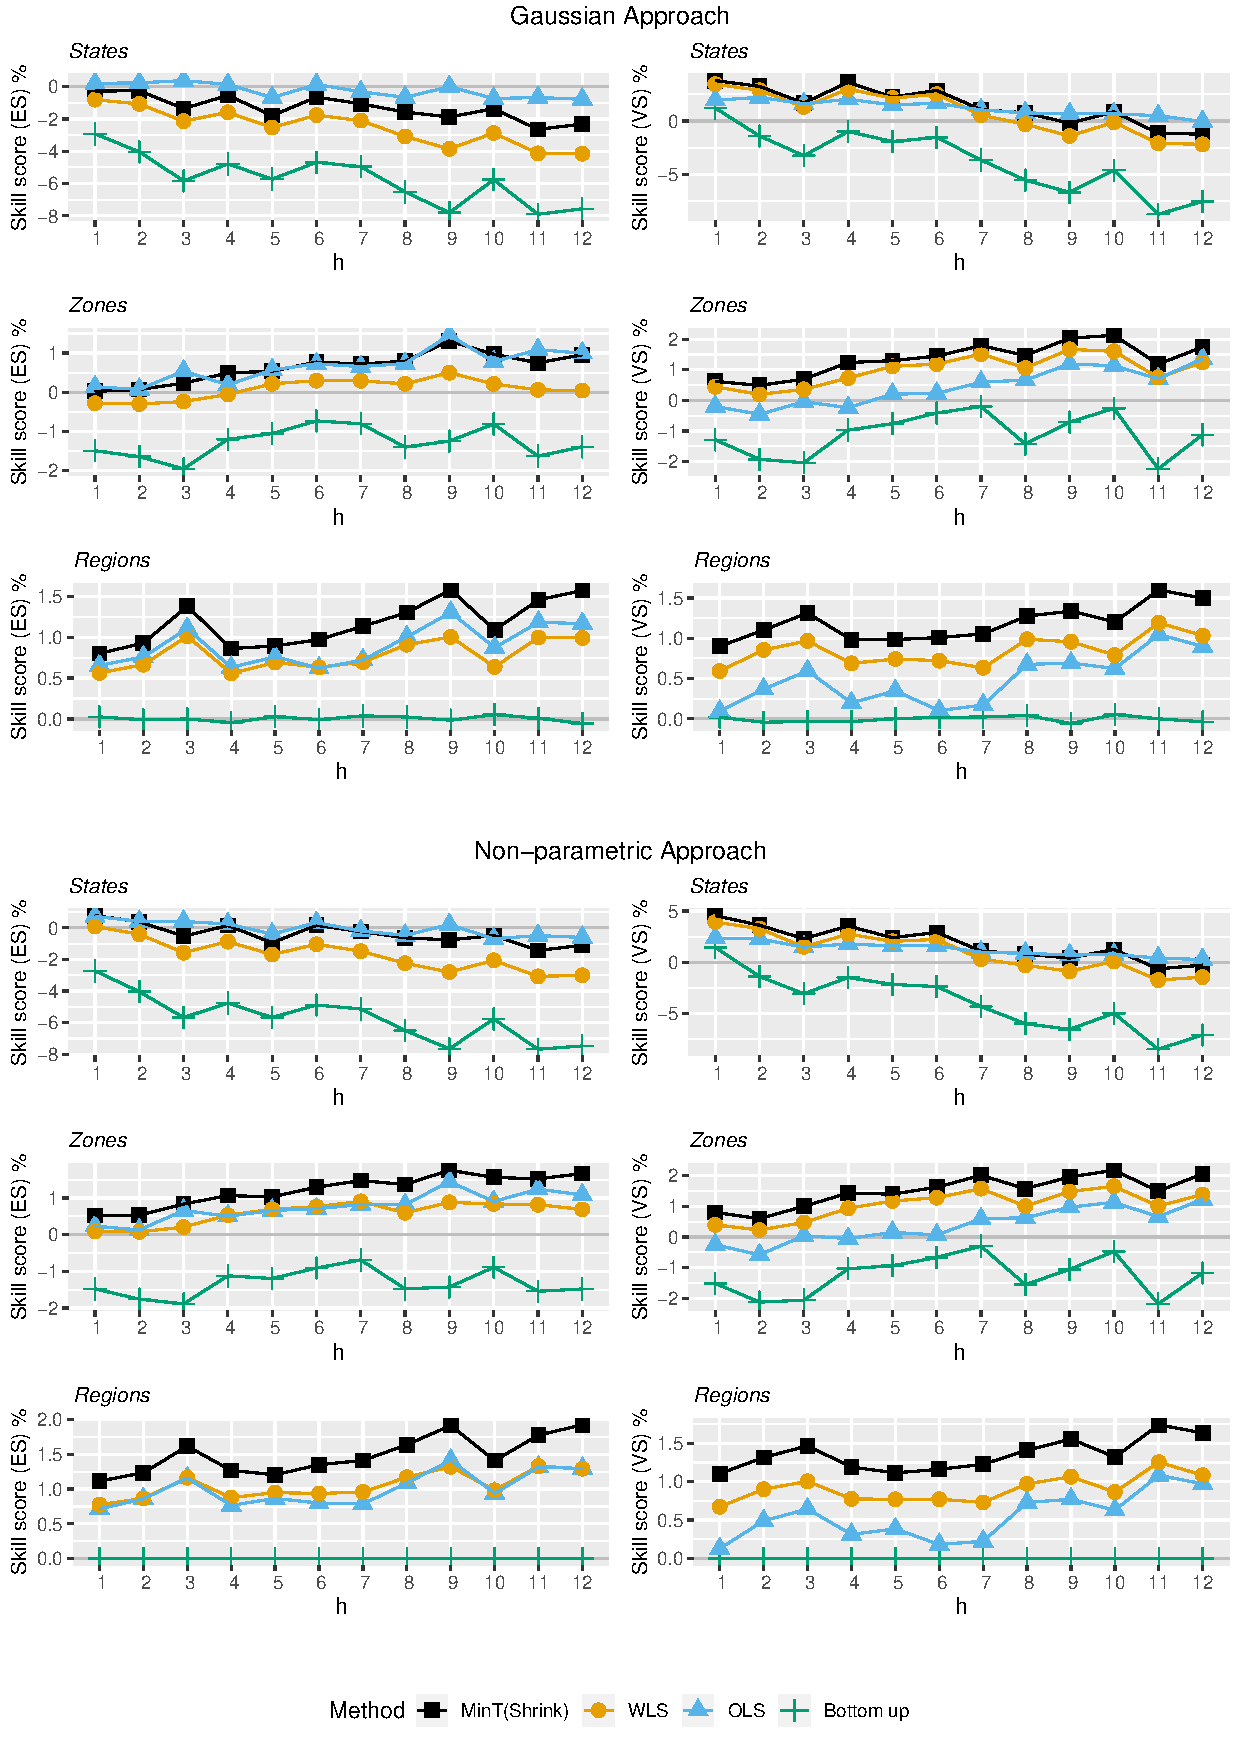
\includegraphics[width= 0.8\textwidth, height= 0.85\textheight]{Empirical-results/Levels_MultiVScores_ETS.pdf}
	\caption{Skill score (with reference to ETS base forecasts) for multivariate probabilistic forecasts of different levels of the hierarchy are presented. Results from Gaussian approach are presented in the top three panels and results from the non-parametric approach are presented in the bottom three panels.}\label{fig:EmpResults_Levels_ETS}
\end{figure}

\begin{figure}[!hbt]
	\centering
	\small
%	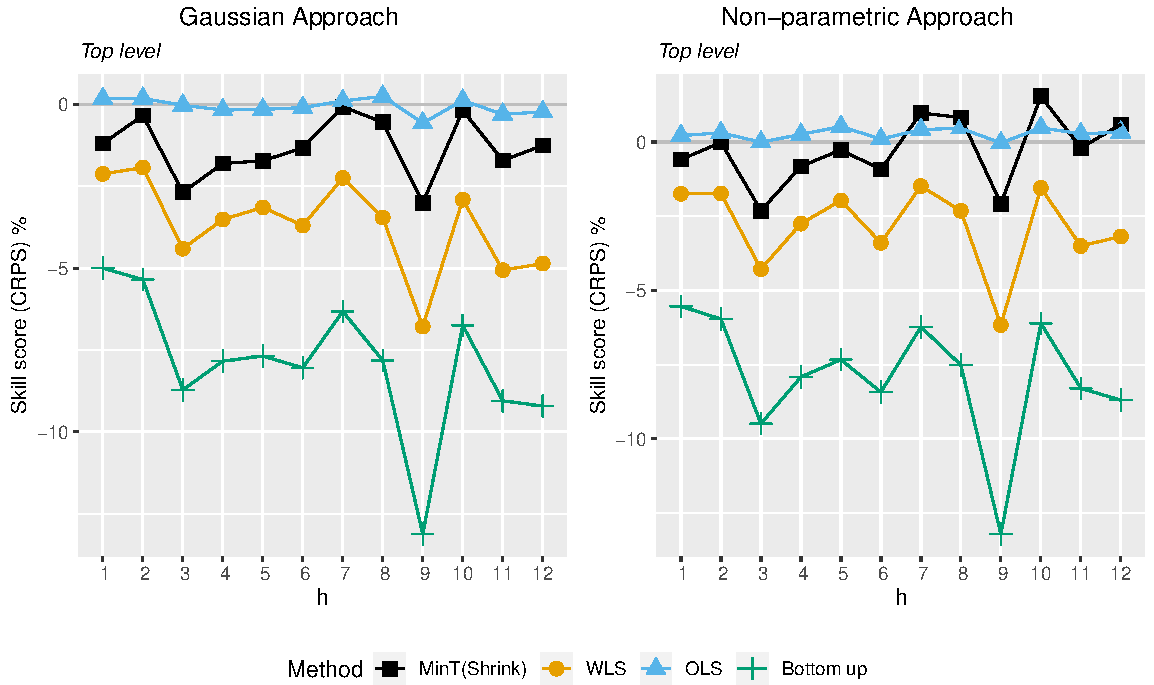
\includegraphics[width= \textwidth]{Empirical-results/UniVScore_TopLevel_ETS.pdf}
	\caption{Skill score based on CRPS (with reference to the ETS base forecasts) for univariate probabilistic forecasts for the Total (top level) overnight trips are presented. Left panel shows the results from Gaussian approach and right panel shows the results from non-parametric approach. }\label{fig:EmpResults_TopLevel_ETS}
\end{figure}

\FloatBarrier

\clearpage

\section{Australian Tourism Hierarchy}\label{app:AustralianData}

Data are collected through the National Visitor Survey managed by Tourism Research Australia based on an annual sample of $120,000$ Australian residents aged $15$ years or more, through telephone interviews \citep{TourismResearch2019}.

\begin{table}[!hb]
	\caption{Geographic hierarchy of Australian tourism flows}\label{tab:AusTourRegions}
	\centering\tabcolsep=0.08cm
	\fontsize{7}{6}\selectfont
	\resizebox{\linewidth}{!}{
		\begin{tabular}{lllllllllll}
			\toprule
			\multicolumn{3}{c}{\textbf{Level 0 - Total}}    &&  \multicolumn{3}{l}{\textit{Regions cont.}}   &  & \multicolumn{3}{l}{\textit{Regions cont.}} \\
			\cmidrule(lr){1-3}
			1 & {\text{Tot}} & {Australia} &&  37	& AAB & Central Coast && 75  & CBD & Mackay   \\
			\cmidrule(lr){1-3}
			\multicolumn{3}{c}{\textbf{Level 1 - States$^*$ }} && 38  & ABA & Hunter && 76 & CBE & Capricorn \\
			\cmidrule(lr){1-3}
			2 & A & NSW 				&  & 39  & ABB & North Coast NSW   && 77 & CBF & Gladstone\\
			3 & B & Victoria 			&  & 40  & ACA & South Coast  && 78  & CCA & Whitsundays\\
			4 & C & Queensland 			&  & 41  & ADA & Snowy Mountains && 79  & CCB & Townsville  \\
			5 & D & South Australia     &  & 42  & ADB & Capital Country && 80  & CCC & Tropical North Queensland   \\
			6 & E & Western Australia   &  & 43  & ADC & The Murray   && 81  & CDA & Southern QLD country\\
			7 & F & Tasmania   			&  & 44  & ADD & Riverina  &&82  & CDB & Outback QLD\\
			8 & G & Northern Territory  &  & 45  & AEA & Central NSW &&83  & DAA & Adelaide   \\
			\cmidrule(lr){1-3}
			\multicolumn{3}{c}{\textbf{Level 2 - Zones}}  &  &  46  & AEB & New England North West && 84  & DAB & Barossa\\
			\cmidrule(lr){1-3}
			9 	& AA & Metro NSW 	  	   	&  & 47  & AEC & Outback NSW   &&85  & DAC & Adelaide Hills\\
			10 	& AB & North Coast NSW 	   	&  & 48  & AED & Blue Mountains  && 86  & DBA & Limestone Coast\\
			11	& AC & South Coast NSW	   	&  & 49  & AFA & Canberra   &&  87  & DBB & Fleurieu Peninsula\\
			12	& AD & South NSW 			&  & 50  & BAA & Melbourne &&88  & DBC & Kangaroo Island\\
			13	& AE & North NSW 			&  & 51  & BAB & Peninsula    &&89  & DCA & Murraylands\\
			14	& AF & ACT					&  &  52  & BAC & Geelong  && 90  & DCB & Riverland\\
			15	& BA & Metro VIC			&  &  53  & BBA & Western   &&91  & DCC & Clare Valley\\
			16	& BB & West Coast VIC		&  &  54  & BCA & Lakes  &&92  & DCD & Flinders Range and Outback\\
			17	& BC & East Coast VIC		&  &  55  & BCB & Gippsland    &&93  & DDA & Eyre Peninsula\\
			18	& BD & North East VIC		&  &  56  & BCC & Phillip Island   &&  94  & DDB & Yorke Peninsula \\
			19	& BE & North West VIC		&  &  57  & BDA & Central Murray    &&95  & EAA & Australia's Coral Coast\\
			20  & CA & Metro QLD			&  & 58  & BDB & Goulburn    &&96  & EAB & Experience Perth\\
			21  & CB & Central Coast QLD	&  & 59  & BDC & High Country   &&97  & EAC & Australia's South West\\
			22  & CC & North Coast QLD		&  &  60  & BDD & Melbourne East &&98  & EBA & Australia's North West \\
			23  & CD & Inland QLD			&  &   61  & BDE & Upper Yarra &&99  & ECA & Australia's Golden Outback\\
			24	& DA & Metro SA				&  & 62  & BDF & Murray East  && 100 & FAA & Hobart and South\\
			25	& DB & South Coast SA		&  &  63  & BEA & Wimmera+Mallee &&101 & FBA & East Coast\\
			26	& DC & Inland SA			&  & 64  & BEB & Western Grampians &&102 & FBB & Launceston, Tamar \& North\\
			27	& DD & West Coast SA		&  &65  & BEC & Bendigo Loddon  &&103 & FCA & North West\\
			
			28	& EA & West Coast WA 	& &  66  & BED & Macedon    &&104 & FCB& West coast\\
			29	& EB & North WA			& &  67  & BEE & Spa Country   &&105 & GAA& Darwin \\
			30	& EC & South WA 		& &   68  & BEF & Ballarat     &&106 & GAB& Litchfield Kakadu Arnhem\\
			31	& FA & South TAS		& &  69  & BEG & Central Highlands  &&107 & GAC& Katherine Daly\\
			32	& FB & North East TAS	& & 70  & CAA & Gold Coast  &&108 & GBA& Barkly\\
			33	& FC & North West TAS	& & 71  & CAB & Brisbane  &&109 & GBB& Lasseter\\
			34	& GA & North Coast NT	& & 72  & CAC & Sunshine Coast &&110 & GBC& Alice Springs\\
			35	& GB & Central NT		& &  73  & CBB & Bundaberg      &&111 & GBD& MacDonnell\\
			\cmidrule(lr){1-3}
			\multicolumn{3}{c}{\textbf{Level 2 - Regions}} & & 74  & CBC & Fraser Coast    &&\\
			\cmidrule(lr){1-3}
			36	& AAA & Sydney 			& 	&  &&\\
			
			\bottomrule
		\end{tabular}
	}
\fontsize{8}{9}\selectfont
$^*$ We consider the Australian Capital Territory as a part of New South Wales and the Northern Territory as a state.
\end{table}


\clearpage
\begin{figure}
	\centering
	\small
	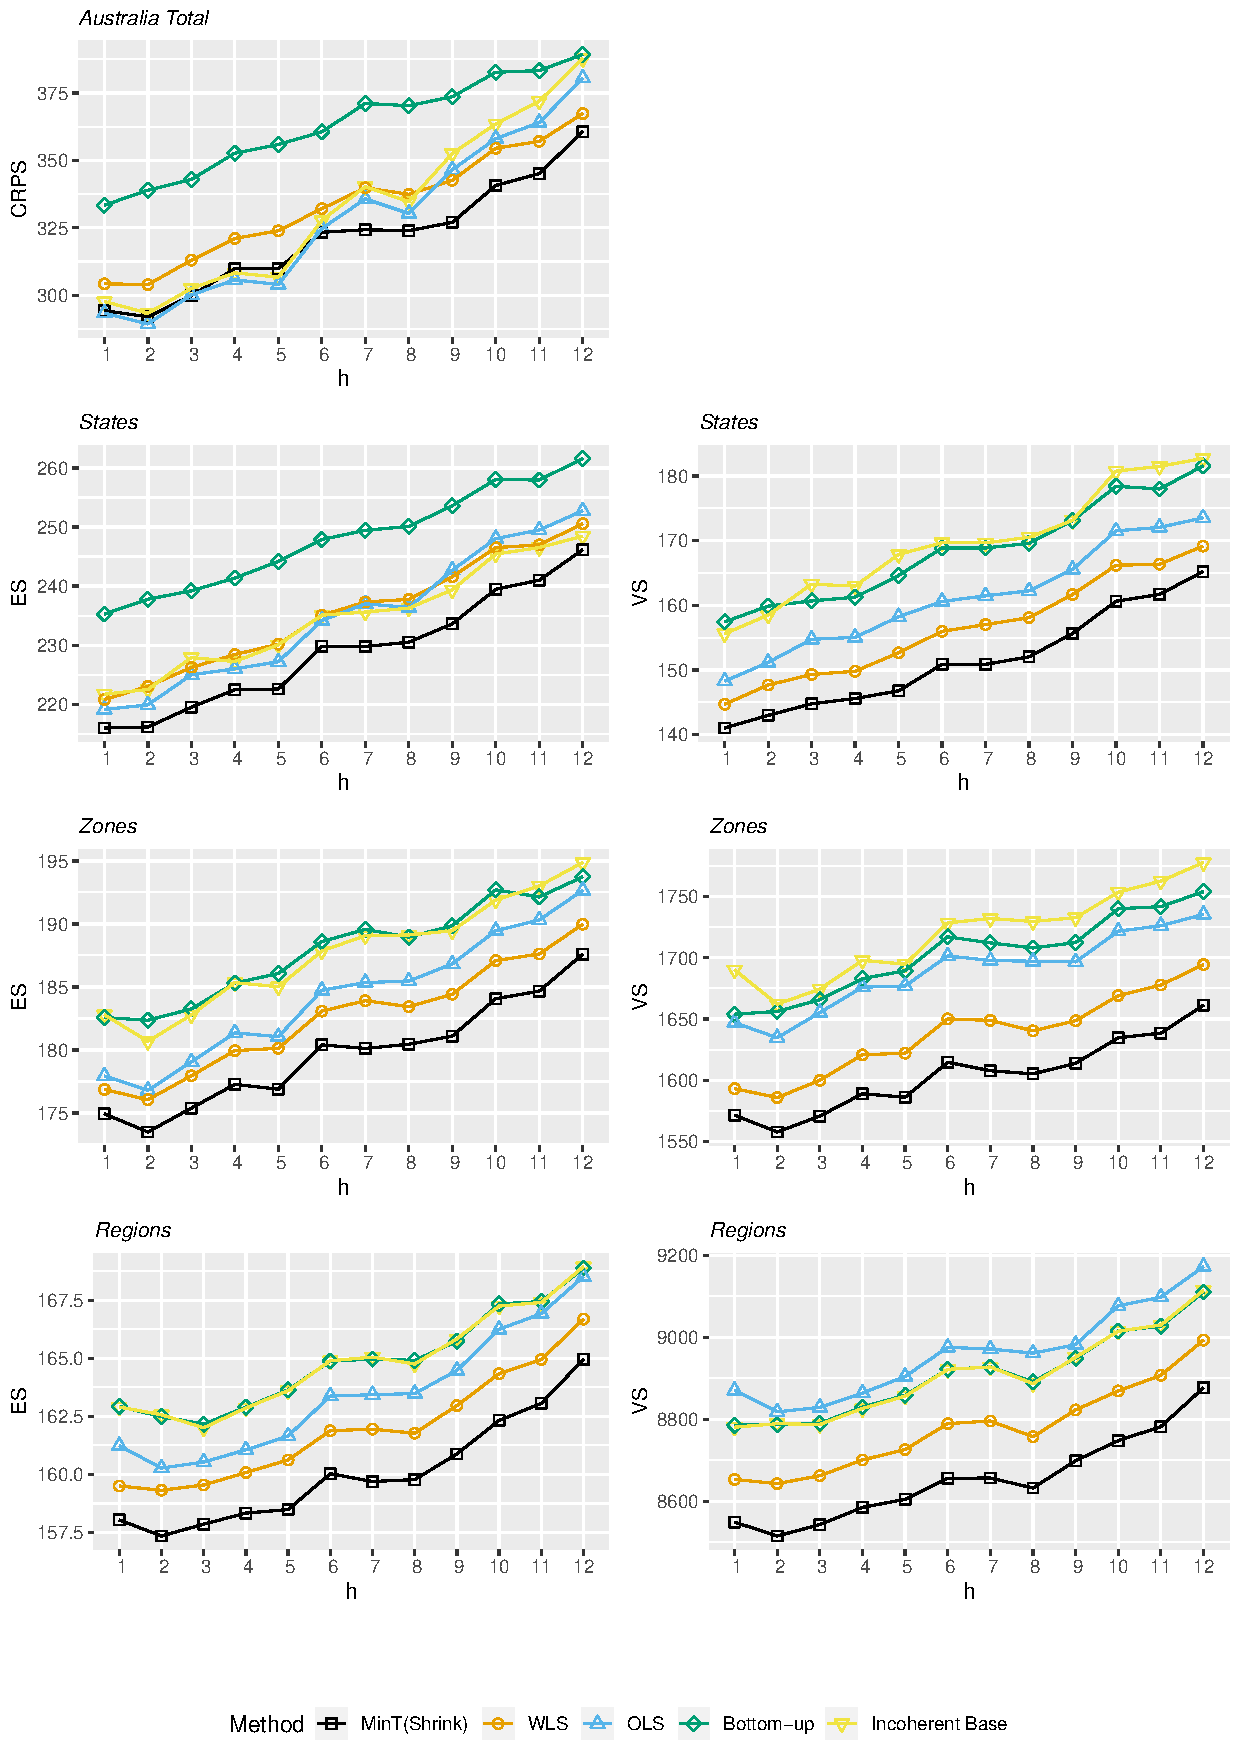
\includegraphics[width= 0.85\textwidth, height= 0.85\textheight]{Empirical-results/Results-ARIMA/RawScore_Gauss_Levels.pdf}
	\caption{Forecast accuracy results across the different levels of the Australia tourism hierarchy. CRPS results are presented for the top-level and energy and variogram scores for the levels below. A lower (higher) score indicates a more (less) accurate forecast. All results are for the analytic solution assuming Gaussian incoherent base forecasts.} \label{fig:ES-Levels}
\end{figure}


\bibliographystyle{agsm}

\bibliography{References_paper2}

\end{document} 